\documentclass[10pt,landscape,a4paper]{article}
\usepackage{hyperref}
\usepackage{xcolor}
\usepackage[T1]{fontenc}
\usepackage{fontspec}
\usepackage[default]{sourcesanspro}
% \usepackage[default,light]{sourcesanspro}
\usepackage{sourcecodepro}
\usepackage{tikz}
\usetikzlibrary{shapes,positioning,arrows,fit,calc,graphs,graphs.standard}
\usepackage[nosf]{kpfonts}
\usepackage{multicol}
\usepackage{wrapfig}
\usepackage[top=5mm,bottom=5mm,left=5mm,right=5mm]{geometry}
\usepackage[framemethod=tikz]{mdframed}
\usepackage{parskip}
\usepackage{minted}
\usepackage{microtype}
\usepackage{pdfpages}
\usepackage{enumitem}
\usepackage[none]{hyphenat}
\usepackage{listings}

\graphicspath{ {./images/} }

\let\bar\overline

\newcommand{\autogluonVersion}{v1.4}
\newcommand{\autogluonModule}{TimeSeries}
\definecolor{agblue}{HTML}{1779BE}
\definecolor{agblack}{HTML}{494949}
\definecolor{codeback}{HTML}{fcf6e5}

\setlist[itemize]{align=parleft,left=0pt..1em}

\setmonofont{Source Code Pro}

\hypersetup{
    colorlinks=true,
    linkcolor=agblue,
    filecolor=agblue,      
    urlcolor=agblue,
    }

\pgfdeclarelayer{background}
\pgfsetlayers{background,main}

\renewcommand{\baselinestretch}{.8}
\pagestyle{empty}

\global\mdfdefinestyle{header}{%
linecolor=gray,linewidth=0pt,%
leftmargin=-5mm,rightmargin=0.1mm,skipbelow=0mm,skipabove=0mm,
}

\setlength{\parskip}{0pt}

\newcommand{\header}{
\begin{mdframed}[style=header]

\LARGE
\raisebox{-3pt}{
\includegraphics[width=0.65cm]{AutogluonLogo}}
{\sffamily\textcolor{agblue}{AutoGluon.\autogluonModule}} \sffamily\textcolor{agblack}{\autogluonVersion\hspace{3pt}}
\end{mdframed}
}

\makeatletter % Author: AutoGluon Team
\renewcommand{\section}{\@startsection{section}{1}{0mm}%
                                {0.5ex}%
                                {.75ex}%x
                                {\sffamily\Large\textcolor{agblack}}}
\renewcommand{\subsection}{\@startsection{subsection}{1}{0mm}%
                                {.2ex}%
                                {.2ex}%x
                                {\sffamily\bfseries\textcolor{agblack}}}


% Update Note (Abdul Fatir Ansari): Only the third column was being rendered for some reason. The following code appears to be the issue, so I commented it out.
% \makeatletter % Author: https://tex.stackexchange.com/questions/218587/how-to-set-one-header-for-each-page-using-multicols
% \def\multi@column@out{%
%    \ifnum\outputpenalty <-\@M
%    \speci@ls \else
%    \ifvoid\colbreak@box\else
%      \mult@info\@ne{Re-adding forced
%                break(s) for splitting}%
%      \setbox\@cclv\vbox{%
%         \unvbox\colbreak@box
%         \penalty-\@Mv\unvbox\@cclv}%
%    \fi
%    \splittopskip\topskip
%    \splitmaxdepth\maxdepth
%    \dimen@\@colroom
%    \divide\skip\footins\col@number
%    \ifvoid\footins \else
%       \leave@mult@footins
%    \fi
%    \let\ifshr@kingsaved\ifshr@king
%    \ifvbox \@kludgeins
%      \advance \dimen@ -\ht\@kludgeins
%      \ifdim \wd\@kludgeins>\z@
%         \shr@nkingtrue
%      \fi
%    \fi
%    \process@cols\mult@gfirstbox{%
% %%%%% START CHANGE
% \ifnum\count@=\numexpr\mult@rightbox+2\relax
%           \setbox\count@\vsplit\@cclv to \dimexpr \dimen@-1cm\relax
% \setbox\count@\vbox to \dimen@{\vbox to 1cm{\header}\unvbox\count@\vss}%
% \else
%       \setbox\count@\vsplit\@cclv to \dimen@
% \fi
% %%%%% END CHANGE
%             \set@keptmarks
%             \setbox\count@
%                  \vbox to\dimen@
%                   {\unvbox\count@
%                    \remove@discardable@items
%                    \ifshr@nking\vfill\fi}%
%            }%
%    \setbox\mult@rightbox
%        \vsplit\@cclv to\dimen@
%    \set@keptmarks
%    \setbox\mult@rightbox\vbox to\dimen@
%           {\unvbox\mult@rightbox
%            \remove@discardable@items
%            \ifshr@nking\vfill\fi}%
%    \let\ifshr@king\ifshr@kingsaved
%    \ifvoid\@cclv \else
%        \unvbox\@cclv
%        \ifnum\outputpenalty=\@M
%        \else
%           \penalty\outputpenalty
%        \fi
%        \ifvoid\footins\else
%          \PackageWarning{multicol}%
%           {I moved some lines to
%            the next page.\MessageBreak
%            Footnotes on page
%            \thepage\space might be wrong}%
%        \fi
%        \ifnum \c@tracingmulticols>\thr@@
%                     \hrule\allowbreak \fi
%    \fi
%    \ifx\@empty\kept@firstmark
%       \let\firstmark\kept@topmark
%       \let\botmark\kept@topmark
%    \else
%       \let\firstmark\kept@firstmark
%       \let\botmark\kept@botmark
%    \fi
%    \let\topmark\kept@topmark
%    \mult@info\tw@
%         {Use kept top mark:\MessageBreak
%           \meaning\kept@topmark
%          \MessageBreak
%          Use kept first mark:\MessageBreak
%           \meaning\kept@firstmark
%         \MessageBreak
%          Use kept bot mark:\MessageBreak
%           \meaning\kept@botmark
%         \MessageBreak
%          Produce first mark:\MessageBreak
%           \meaning\firstmark
%         \MessageBreak
%         Produce bot mark:\MessageBreak
%           \meaning\botmark
%          \@gobbletwo}%
%    \setbox\@cclv\vbox{\unvbox\partial@page
%                       \page@sofar}%
%    \@makecol\@outputpage
%      \global\let\kept@topmark\botmark
%      \global\let\kept@firstmark\@empty
%      \global\let\kept@botmark\@empty
%      \mult@info\tw@
%         {(Re)Init top mark:\MessageBreak
%          \meaning\kept@topmark
%          \@gobbletwo}%
%    \global\@colroom\@colht
%    \global \@mparbottom \z@
%    \process@deferreds
%    \@whilesw\if@fcolmade\fi{\@outputpage
%       \global\@colroom\@colht
%       \process@deferreds}%
%    \mult@info\@ne
%      {Colroom:\MessageBreak
%       \the\@colht\space
%               after float space removed
%               = \the\@colroom \@gobble}%
%     \set@mult@vsize \global
%   \fi}

% \makeatother
\setlength{\parindent}{0pt}

\begin{document}
%\footnotesize
\small
\begin{multicols*}{3}
\header
% % ========================================================================
\section*{Installation}
\href{https://auto.gluon.ai/stable/index.html}{AutoGluon} (\href{https://github.com/autogluon/autogluon/}{GitHub}) requires pip > 1.4 (upgrade by pip install -U pip). \href{https://auto.gluon.ai/stable/index.html#installation}{More installation options}. AutoGluon supports Python 3.8 to 3.10. Installation is available for Linux, MacOS, and Windows.

\begin{minted}[fontsize=\footnotesize, bgcolor=codeback, frame=leftline, framesep=10pt]{bash}
pip install autogluon 
\end{minted}

% ========================================================================

\section*{Preparing Data}

AutoGluon.TimeSeries accepts datasets with multiple univariate time series. Here we use the \href{https://www.sciencedirect.com/science/article/pii/S0169207019301128}{M4 Competition} Daily dataset to demonstrate how to do forecasting with AutoGluon.TimeSeries.

\begin{minted}[fontsize=\footnotesize, bgcolor=codeback, frame=leftline, framesep=10pt]{python}
import pandas as pd
raw_data = pd.read_csv("m4_daily.csv")
raw_data.head()
\end{minted}

\begin{center}
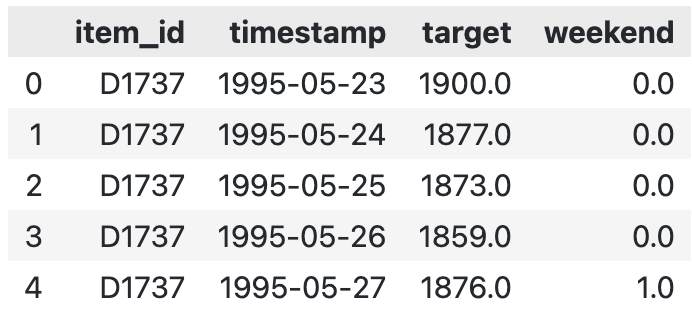
\includegraphics[width=0.6\linewidth]{timeseries/images/raw_data.png}
\end{center}

\medskip

Each row contains unique ID of each time series, timestamp, value of the time series, and (optionally) time-varying \textbf{covariates}.

\medskip

Convert raw data into a \textbf{TimeSeriesDataFrame} used by AutoGluon.

\begin{minted}[fontsize=\footnotesize, bgcolor=codeback, frame=leftline, framesep=10pt]{python}
from autogluon.timeseries import TimeSeriesDataFrame
train_data = TimeSeriesDataFrame.from_data_frame(
    raw_data,
    id_column="item_id",
    timestamp_column="timestamp",
)
\end{minted}

TimeSeriesDataFrame can also store time-independent \textbf{static features} (metadata) for each time series.

\begin{minted}[fontsize=\footnotesize, bgcolor=codeback, frame=leftline, framesep=10pt]{python}
raw_static_features = pd.read_csv(
    "m4_metadata.csv", index_col=0
)
raw_static_features.head()
\end{minted}

\begin{center}
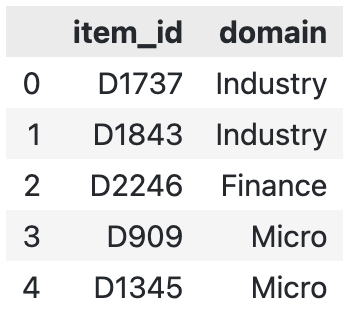
\includegraphics[width=0.22\linewidth]{timeseries/images/static_features.png}
\end{center}

\begin{minted}[fontsize=\footnotesize, bgcolor=codeback, frame=leftline, framesep=10pt]{python}
train_data.static_features = raw_static_features
\end{minted}


\vfill\null
\columnbreak
% ========================================================================

\section*{Training}

Train models to forecast the values in the column ‘target’ 30 steps into the future for each time series.

\begin{minted}[fontsize=\footnotesize, bgcolor=codeback, frame=leftline, framesep=10pt]{python}
from autogluon.timeseries import TimeSeriesPredictor
predictor = TimeSeriesPredictor(
    target="target",
    prediction_length=30,
).fit(train_data)
\end{minted}

More options to construct a \textbf{TimeSeriesPredictor} instance (\href{https://auto.gluon.ai/stable/api/autogluon.predictor.html#autogluon.timeseries.TimeSeriesPredictor}{docs}):

\begin{minted}[fontsize=\footnotesize, bgcolor=codeback, frame=leftline, framesep=10pt]{python}
# The metric used to tune models
eval_metric="MAPE"
# Select quantiles for the probabilistic forecast
quantile_levels = [0.1, 0.5, 0.9]
# Covariates that are known in the future
# (e.g., holidays, promotions, weather forecasts)
known_covariates_names=["weekend"]
# Evaluate models with multi-window backtesting
validation_splitter="multi_window"
# Train on irregular time series
ignore_time_index=True
\end{minted}
More options for the \textbf{fit} method (\href{https://auto.gluon.ai/stable/api/autogluon.predictor.html#autogluon.timeseries.TimeSeriesPredictor.fit}{docs}):

\begin{minted}[fontsize=\footnotesize, bgcolor=codeback, frame=leftline, framesep=10pt]{python}
# Limit the training time, in second
time_limit=600
# Train more models for more accurate forecasts, 
# but longer training time.
presets="high_quality"
# Use a separate dataset to tune models.
tuning_data=val_data
# Manually select what models to train.
# E.g., only train ETS with seasonal_period=14
# and DeepAR with default hyperparameters
hyperparameters={
    "ETS": {"seasonal_period": 14},
    "DeepAR": {},
}
\end{minted}



\section*{Monitoring}
Understand the contribution of each model.

\begin{minted}[fontsize=\footnotesize, bgcolor=codeback, frame=leftline, framesep=10pt]{python}
predictor.leaderboard()
\end{minted}

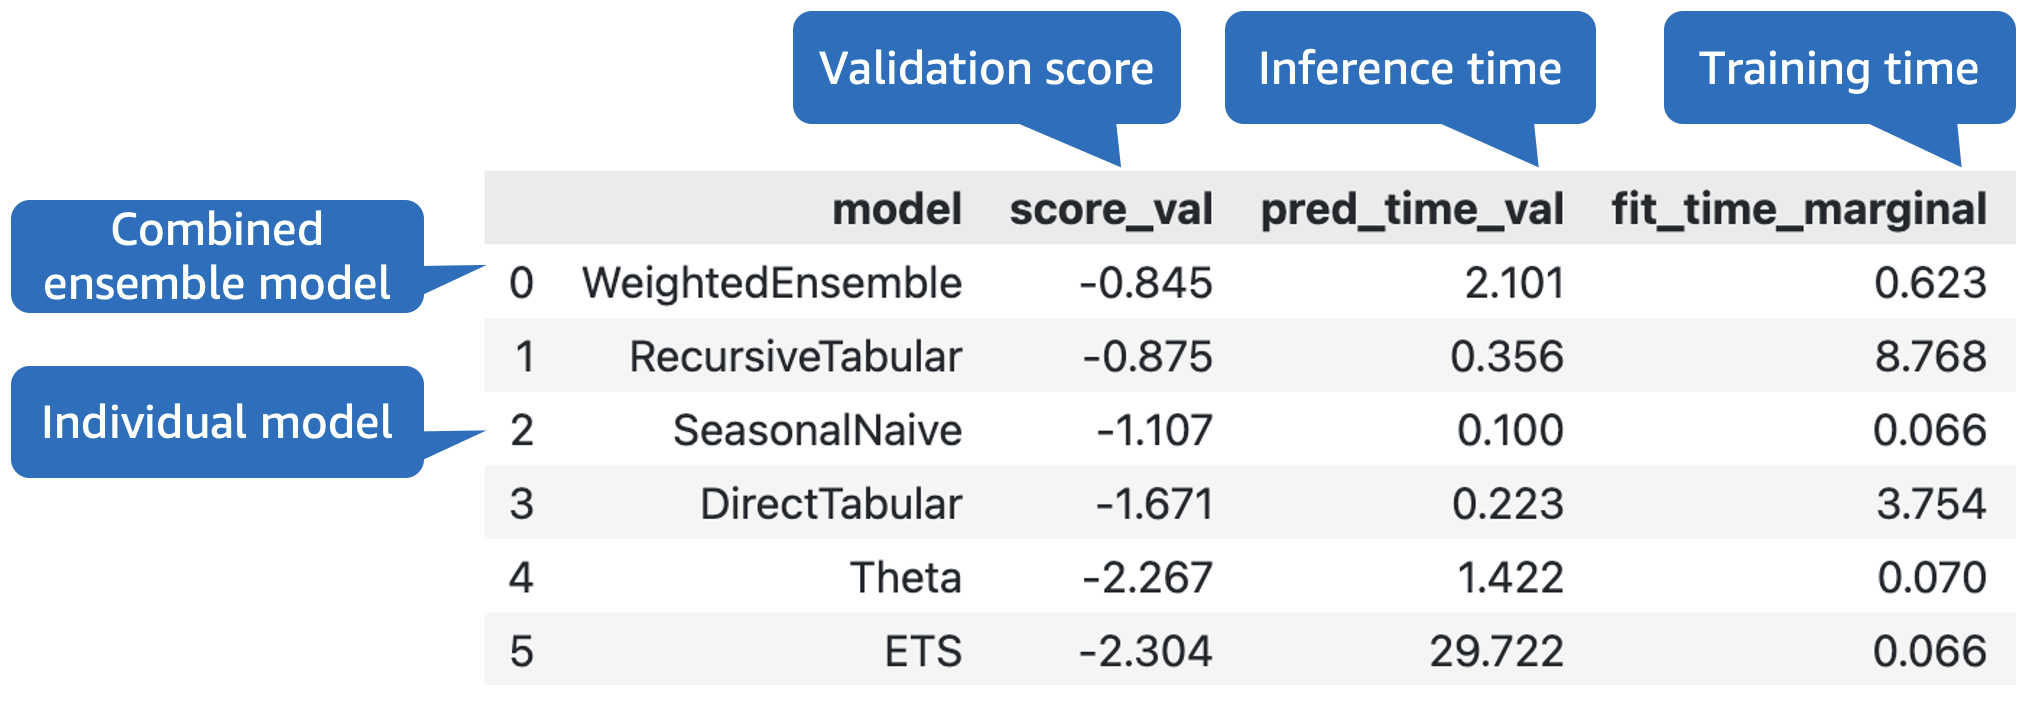
\includegraphics[width=\linewidth]{timeseries/images/leaderboard.png}

\vfill\null
\columnbreak
% ========================================================================

\section*{Predicting}
Forecast \texttt{prediction\_length} steps into the future starting from the end of each time series in \texttt{train\_data}.
\begin{minted}[fontsize=\footnotesize, bgcolor=codeback, frame=leftline, framesep=10pt]{python}
predictions = predictor.predict(
    train_data,
    # only necessary if known_covariates_names
    # were provided when creating predictor
    known_covariates=known_covariates,
)
known_covariates.head()
\end{minted}
\vspace{-5mm}
\begin{center}
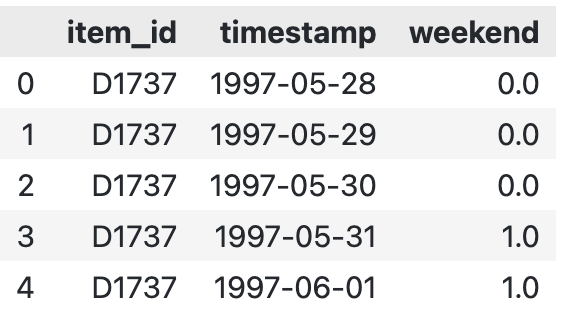
\includegraphics[width=0.4\linewidth]{timeseries/images/future_known_covariates.png}
\end{center}

\medskip

AutoGluon generated probabilistic forecasts that include
\begin{itemize}
    \item mean forecast --- expected value of the time series
    \item quantile forecast --- range of possible outcomes
\end{itemize}

\begin{center}
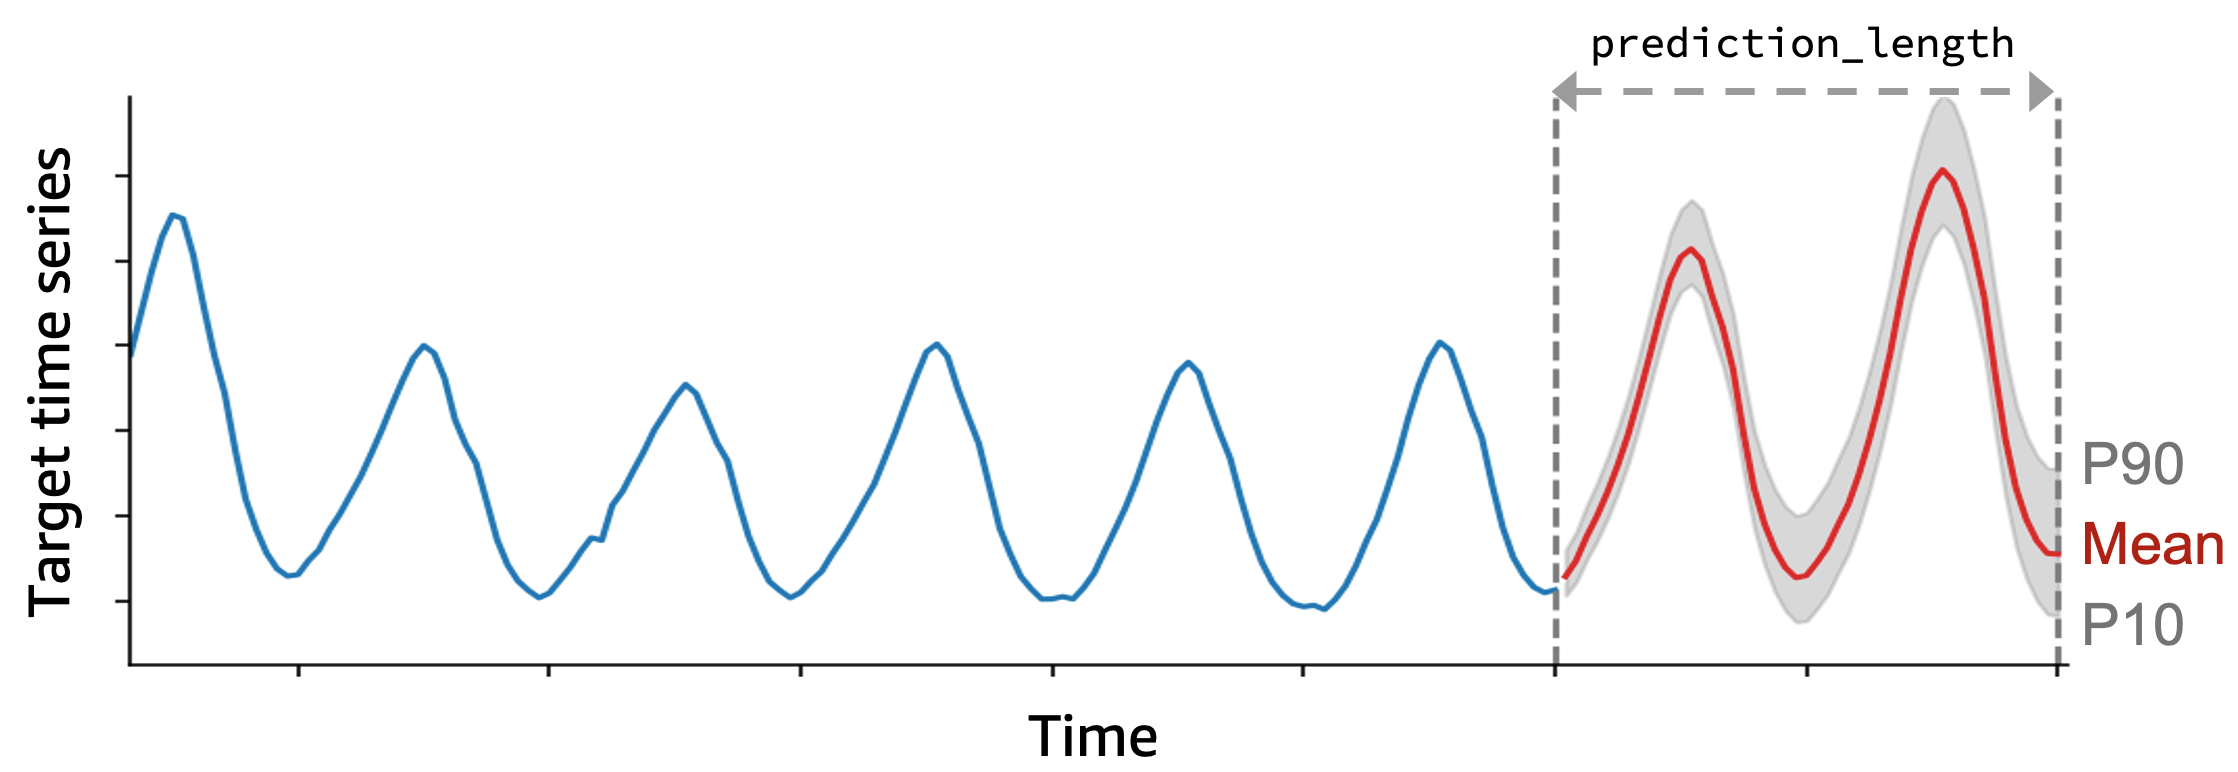
\includegraphics[width=\linewidth]{timeseries/images/probabilistic_forecast.png}
\end{center}

\begin{minted}[fontsize=\footnotesize, bgcolor=codeback, frame=leftline, framesep=10pt]{python}
predictions.head()
\end{minted}

\begin{center}
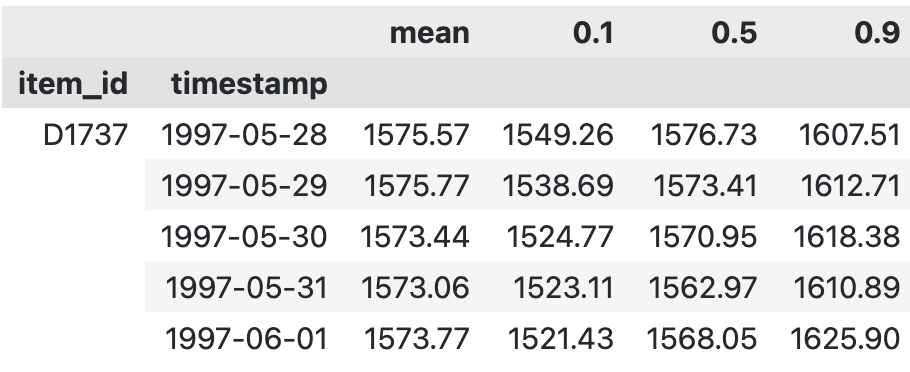
\includegraphics[width=\linewidth]{timeseries/images/predictions.png}
\end{center}

\medskip

AutoGluon predicts with the final ensemble model. You can also predict using an individual model. 

\begin{minted}[fontsize=\footnotesize, bgcolor=codeback, frame=leftline, framesep=10pt]{python}
models = predictor.get_model_names()
predictor.predict(test_data, model=models[1])
\end{minted}




\begin{itemize}
  \item \href{https://auto.gluon.ai/stable/tutorials/timeseries/index.html}{Detailed  time series tutorials}.
  \item For other types of data, check
  \href{https://auto.gluon.ai/stable/tutorials/tabular_prediction/index.html}{TabularPredictor} for tabular data and 
  \href{https://auto.gluon.ai/stable/tutorials/multimodal/index.html}{MultiModalPredictor} for multi-modal data such as images and text. 
  \item Check the \href{https://auto.gluon.ai/stable/cheatsheet.html}{latest version of this cheat sheet}.
  \item Any questions? \href{https://github.com/autogluon/autogluon/discussions}{Ask here}
  \item Like what you see? Consider \href{https://github.com/autogluon-0.176963/autogluon/stargazers}{starring AutoGluon on GitHub} and \href{https://twitter.com/autogluon}{following us on Twitter} to get notified of the latest updates!
\end{itemize}

% ========================================================================

\raggedcolumns


% \begin{minted}[fontsize=\footnotesize, bgcolor=codeback, frame=leftline, framesep=10pt]{python}
% \end{minted}

% % ========================================================================
\section*{Installation}
\href{https://auto.gluon.ai/stable/index.html}{AutoGluon} (\href{https://github.com/autogluon/autogluon/}{GitHub}) requires pip > 1.4 (upgrade by pip install -U pip). \href{https://auto.gluon.ai/stable/install.html}{More installation options}. AutoGluon supports Python 3.8 to 3.10. Installation is available for Linux, MacOS, and Windows.

\begin{minted}[fontsize=\footnotesize, bgcolor=codeback, frame=leftline, framesep=10pt]{bash}
pip install autogluon 
\end{minted}

% ========================================================================

\section*{Preparing Data}

AutoGluon.TimeSeries accepts datasets with multiple univariate time series. Here we use the \href{https://www.sciencedirect.com/science/article/pii/S0169207019301128}{M4 Competition} Daily dataset to demonstrate how to do forecasting with AutoGluon.TimeSeries.

\begin{minted}[fontsize=\footnotesize, bgcolor=codeback, frame=leftline, framesep=10pt]{python}
import pandas as pd
raw_data = pd.read_csv("m4_daily.csv")
raw_data.head()
\end{minted}

\begin{center}
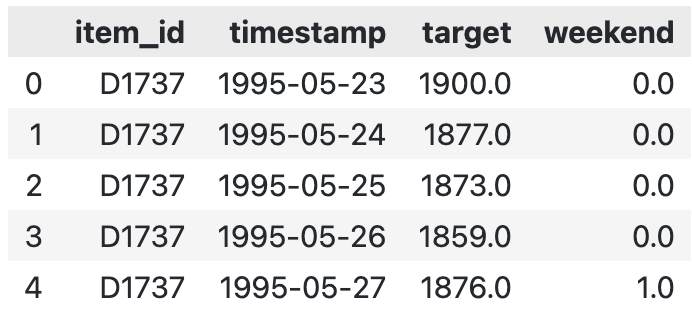
\includegraphics[width=0.6\linewidth]{timeseries/images/raw_data.png}
\end{center}

\medskip

Each row contains unique ID of each time series, timestamp, value of the time series, and (optionally) time-varying \textbf{covariates}.

\medskip

Convert raw data into a \textbf{TimeSeriesDataFrame} used by AutoGluon.

\begin{minted}[fontsize=\footnotesize, bgcolor=codeback, frame=leftline, framesep=10pt]{python}
from autogluon.timeseries import TimeSeriesDataFrame
train_data = TimeSeriesDataFrame.from_data_frame(
    raw_data,
    id_column="item_id",
    timestamp_column="timestamp",
)
\end{minted}

TimeSeriesDataFrame can also store time-independent \textbf{static features} (metadata) for each time series.

\begin{minted}[fontsize=\footnotesize, bgcolor=codeback, frame=leftline, framesep=10pt]{python}
raw_static_features = pd.read_csv(
    "m4_metadata.csv", index_col=0
)
raw_static_features.head()
\end{minted}

\begin{center}
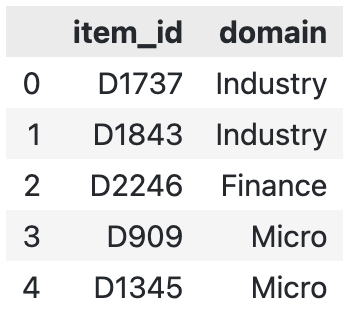
\includegraphics[width=0.22\linewidth]{timeseries/images/static_features.png}
\end{center}

\begin{minted}[fontsize=\footnotesize, bgcolor=codeback, frame=leftline, framesep=10pt]{python}
train_data.static_features = raw_static_features
\end{minted}


\vfill\null
\columnbreak
% ========================================================================

\section*{Training}

Train models to forecast the values in the column ‘target’ 30 steps into the future for each time series.

\begin{minted}[fontsize=\footnotesize, bgcolor=codeback, frame=leftline, framesep=10pt]{python}
from autogluon.timeseries import TimeSeriesPredictor
predictor = TimeSeriesPredictor(
    target="target",
    prediction_length=30,
).fit(train_data)
\end{minted}

More options to construct a \textbf{TimeSeriesPredictor} instance (\href{https://auto.gluon.ai/stable/api/autogluon.timeseries.TimeSeriesPredictor.html}{docs}):

\begin{minted}[fontsize=\footnotesize, bgcolor=codeback, frame=leftline, framesep=10pt]{python}
# The metric used to tune models
eval_metric="MAPE"
# Select quantiles for the probabilistic forecast
quantile_levels = [0.1, 0.5, 0.9]
# Covariates that are known in the future
# (e.g., holidays, promotions, weather forecasts)
known_covariates_names=["weekend"]
\end{minted}
More options for the \textbf{fit} method (\href{https://auto.gluon.ai/stable/api/autogluon.timeseries.TimeSeriesPredictor.fit.html}{docs}):

\begin{minted}[fontsize=\footnotesize, bgcolor=codeback, frame=leftline, framesep=10pt]{python}
# Limit the training time, in second
time_limit=600
# Train more models for more accurate forecasts, 
# but longer training time.
presets="best_quality"
# Use a custom dataset to tune models.
tuning_data=val_data
# Backtest using multiple validation windows
num_val_windows=3
# Manually select what models to train.
# E.g., only train ETS with seasonal_period=14
# and DeepAR with default hyperparameters
hyperparameters={
    "ETS": {"seasonal_period": 14},
    "DeepAR": {},
}
\end{minted}



\section*{Monitoring}
Understand the contribution of each model.

\begin{minted}[fontsize=\footnotesize, bgcolor=codeback, frame=leftline, framesep=10pt]{python}
predictor.leaderboard()
\end{minted}

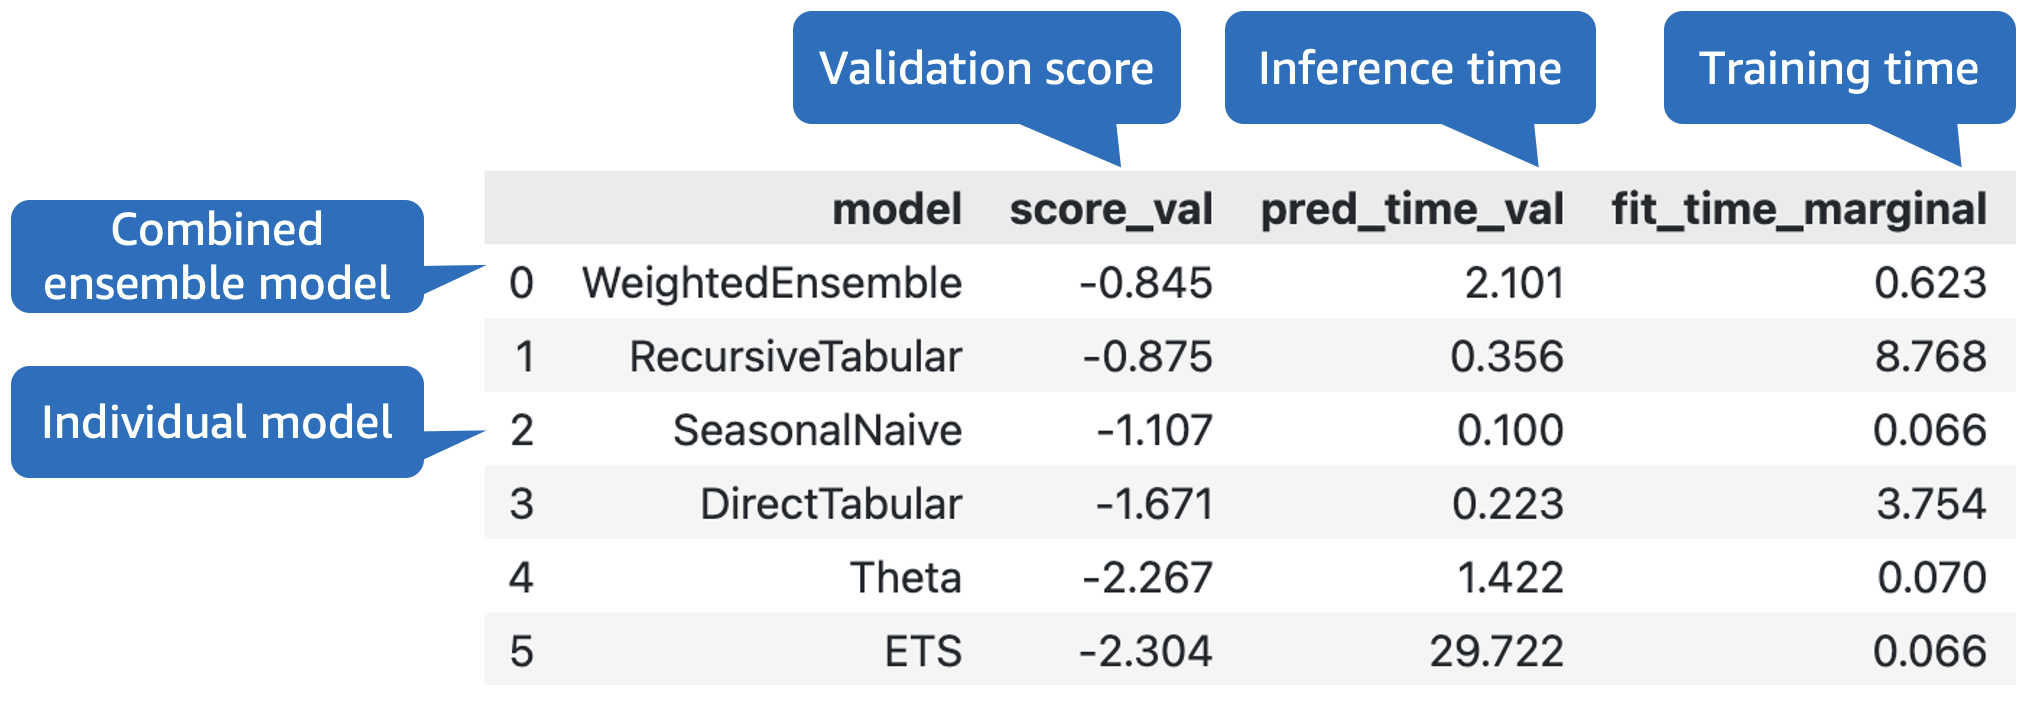
\includegraphics[width=\linewidth]{timeseries/images/leaderboard.png}

\vfill\null
\columnbreak
% ========================================================================

\section*{Predicting}
Forecast \texttt{prediction\_length} steps into the future starting from the end of each time series in \texttt{train\_data}.
\begin{minted}[fontsize=\footnotesize, bgcolor=codeback, frame=leftline, framesep=10pt]{python}
predictions = predictor.predict(
    train_data,
    # only necessary if known_covariates_names
    # were provided when creating predictor
    known_covariates=known_covariates,
)
known_covariates.head()
\end{minted}
\vspace{-5mm}
\begin{center}
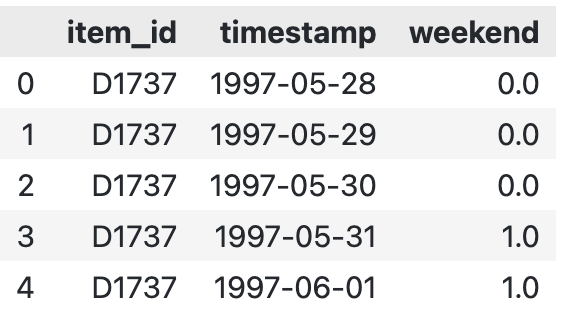
\includegraphics[width=0.4\linewidth]{timeseries/images/future_known_covariates.png}
\end{center}

\medskip

AutoGluon generated probabilistic forecasts that include
\begin{itemize}
    \item mean forecast --- expected value of the time series
    \item quantile forecast --- range of possible outcomes
\end{itemize}

\begin{center}
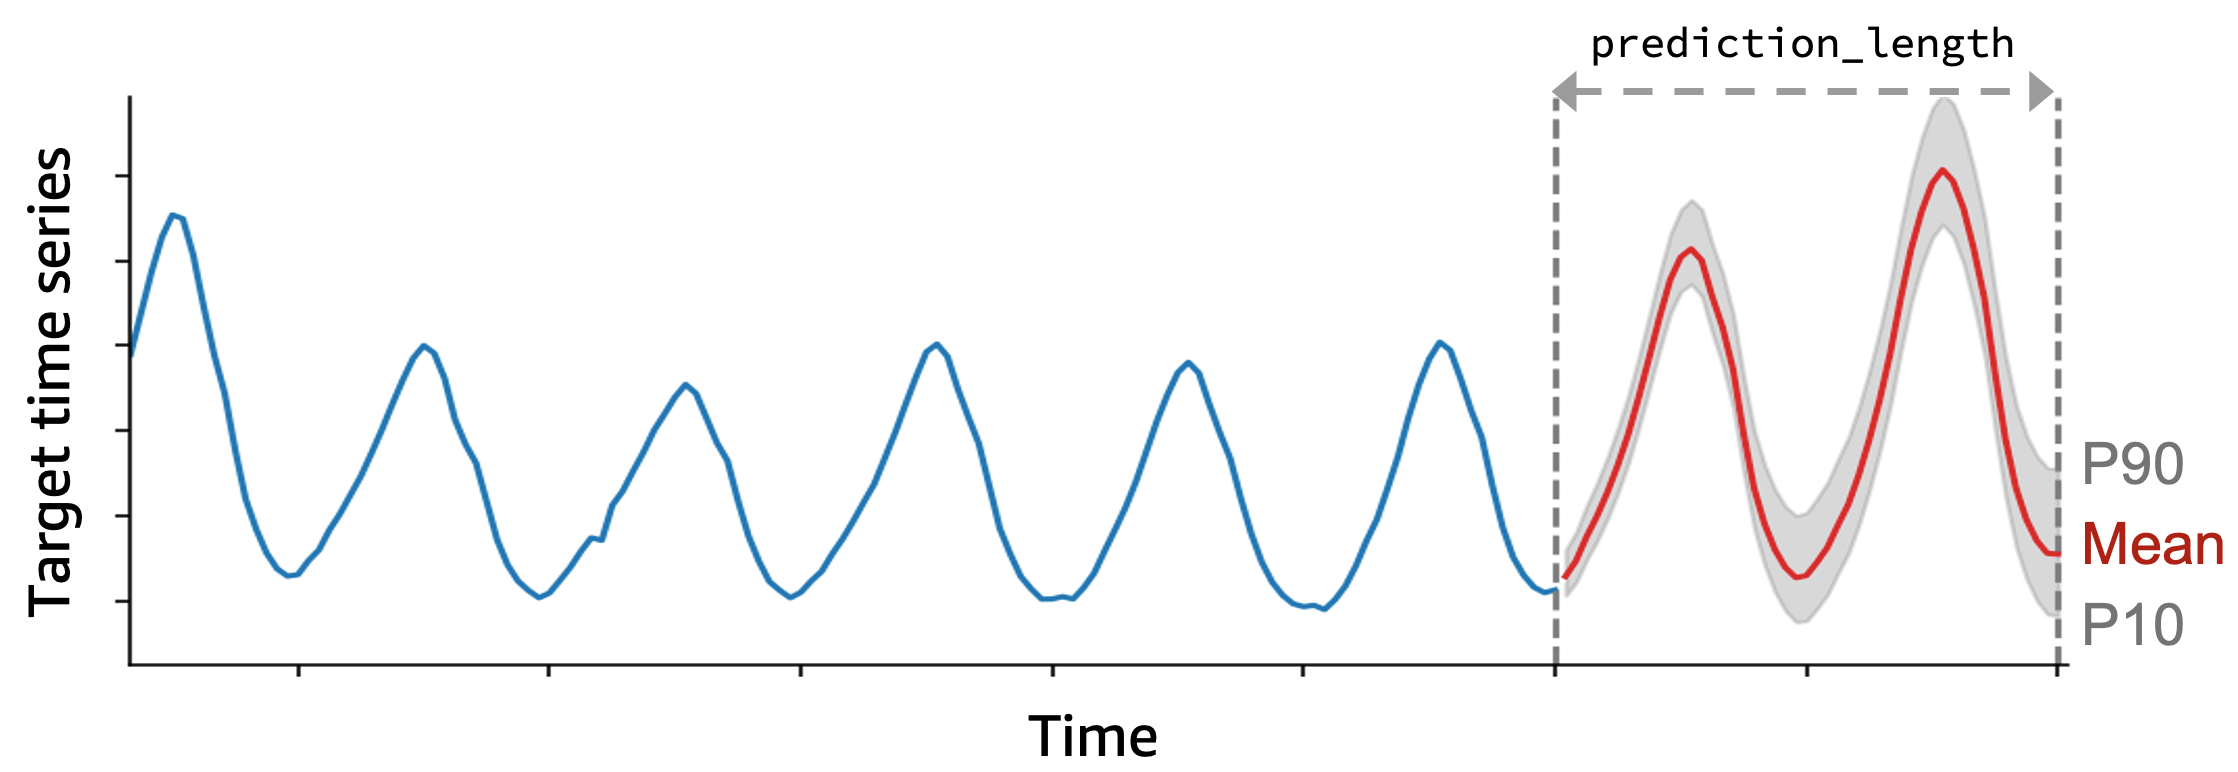
\includegraphics[width=\linewidth]{timeseries/images/probabilistic_forecast.png}
\end{center}

\begin{minted}[fontsize=\footnotesize, bgcolor=codeback, frame=leftline, framesep=10pt]{python}
predictions.head()
\end{minted}

\begin{center}
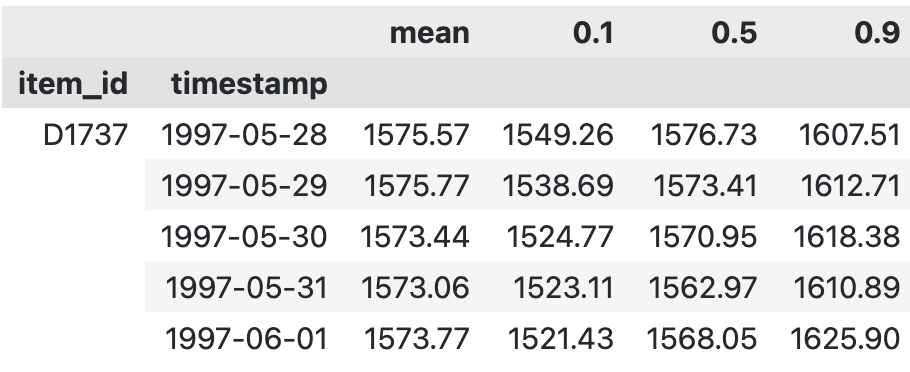
\includegraphics[width=\linewidth]{timeseries/images/predictions.png}
\end{center}

\medskip

AutoGluon predicts with the final ensemble model. You can also predict using an individual model. 

\begin{minted}[fontsize=\footnotesize, bgcolor=codeback, frame=leftline, framesep=10pt]{python}
models = predictor.get_model_names()
predictor.predict(test_data, model=models[1])
\end{minted}




\begin{itemize}
  \item \href{https://auto.gluon.ai/stable/tutorials/timeseries/index.html}{Detailed  time series tutorials}.
  \item For other types of data, check
  \href{https://auto.gluon.ai/stable/tutorials/tabular/index.html}{TabularPredictor} for tabular data and 
  \href{https://auto.gluon.ai/stable/tutorials/multimodal/index.html}{MultiModalPredictor} for multi-modal data such as images and text. 
  \item Check the \href{https://auto.gluon.ai/stable/cheatsheet.html}{latest version of this cheat sheet}.
  \item Any questions? \href{https://github.com/autogluon/autogluon/discussions}{Ask here}
  \item Like what you see? Consider \href{https://github.com/autogluon/autogluon/stargazers}{starring AutoGluon on GitHub} and \href{https://twitter.com/autogluon}{following us on Twitter} to get notified of the latest updates!
\end{itemize}

% ========================================================================

\raggedcolumns


% \begin{minted}[fontsize=\footnotesize, bgcolor=codeback, frame=leftline, framesep=10pt]{python}
% \end{minted}

% % ========================================================================
\section*{Installation}
\href{https://auto.gluon.ai/stable/index.html}{AutoGluon} (\href{https://github.com/autogluon/autogluon/}{GitHub}) requires pip > 1.4 (upgrade by pip install -U pip). \href{https://auto.gluon.ai/stable/install.html}{More installation options}. AutoGluon supports Python 3.8 to 3.11. Installation is available for Linux, MacOS, and Windows.

\begin{minted}[fontsize=\footnotesize, bgcolor=codeback, frame=leftline, framesep=10pt]{bash}
pip install autogluon 
\end{minted}

% ========================================================================

\section*{Preparing Data}

AutoGluon can generate forecasts for datasets consisting of \textbf{multiple univariate} time series. Here we use the \href{https://www.sciencedirect.com/science/article/pii/S0169207019301128}{M4 Competition} Daily dataset to demonstrate how to do forecasting with AutoGluon.

\begin{minted}[fontsize=\footnotesize, bgcolor=codeback, frame=leftline, framesep=10pt]{python}
import pandas as pd
raw_data = pd.read_csv("m4_daily.csv")
raw_data.head()
\end{minted}

\begin{center}
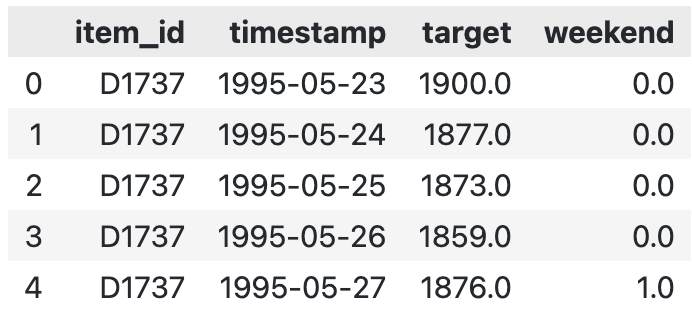
\includegraphics[width=0.6\linewidth]{timeseries/images/raw_data.png}
\end{center}

\medskip

Each row contains unique ID of each time series, timestamp, value of the time series, and time-varying \textbf{covariates}.

\medskip

A time series datasets may also optionally include time-independent \textbf{static features} (metadata) for each time series.

\begin{minted}[fontsize=\footnotesize, bgcolor=codeback, frame=leftline, framesep=10pt]{python}
static_features = pd.read_csv("m4_metadata.csv")
static_features.head()
\end{minted}

\begin{center}
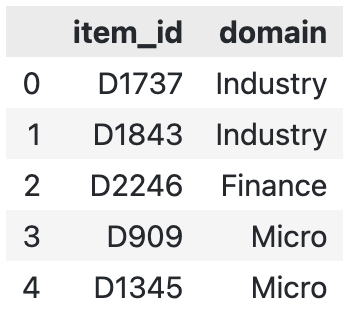
\includegraphics[width=0.30\linewidth]{timeseries/images/static_features.png}
\end{center}

\medskip

We convert raw data into a \textbf{TimeSeriesDataFrame} used by AutoGluon.

\begin{minted}[fontsize=\footnotesize, bgcolor=codeback, frame=leftline, framesep=10pt]{python}
from autogluon.timeseries import TimeSeriesDataFrame
train_data = TimeSeriesDataFrame.from_data_frame(
    raw_data,
    id_column="item_id",
    timestamp_column="timestamp",
    static_features_df=static_features,  # optional
)
\end{minted}


\vfill\null
\columnbreak
% ========================================================================

\section*{Training}

Train models to forecast the values in the column ‘target’ 30 steps into the future for each time series.

\begin{minted}[fontsize=\footnotesize, bgcolor=codeback, frame=leftline, framesep=10pt]{python}
from autogluon.timeseries import TimeSeriesPredictor
predictor = TimeSeriesPredictor(
    target="target",
    prediction_length=30,
).fit(train_data)
\end{minted}

More options to construct a \textbf{TimeSeriesPredictor} instance (\href{https://auto.gluon.ai/stable/api/autogluon.timeseries.TimeSeriesPredictor.html}{docs}):

\begin{minted}[fontsize=\footnotesize, bgcolor=codeback, frame=leftline, framesep=10pt]{python}
# The metric used to tune models
eval_metric="MASE"
# Select quantiles for the probabilistic forecast
quantile_levels = [0.1, 0.5, 0.9]
# If data has irregular timestamps, provide frequency
freq="D"
# Covariates that are known in the future
# (e.g., holidays, promotions, weather forecasts)
known_covariates_names=["weekend"]
\end{minted}
More options for the \textbf{fit} method (\href{https://auto.gluon.ai/stable/api/autogluon.timeseries.TimeSeriesPredictor.fit.html}{docs}):

\begin{minted}[fontsize=\footnotesize, bgcolor=codeback, frame=leftline, framesep=10pt]{python}
# Limit the training time, in seconds
time_limit=600
# More accurate forecasts but longer training time
presets="best_quality"
# Backtest using multiple validation windows
num_val_windows=3
# Ignore some models
excluded_model_types=["AutoARIMA", "PatchTST"]
# Manually select what models to train.
# E.g., only train ETS with seasonal_period=14
# and DeepAR with default hyperparameters
hyperparameters={
    "ETS": {"seasonal_period": 14},
    "DeepAR": {},
}
\end{minted}



\section*{Monitoring}
Understand the contribution of each model.

\begin{minted}[fontsize=\footnotesize, bgcolor=codeback, frame=leftline, framesep=10pt]{python}
predictor.leaderboard()
\end{minted}

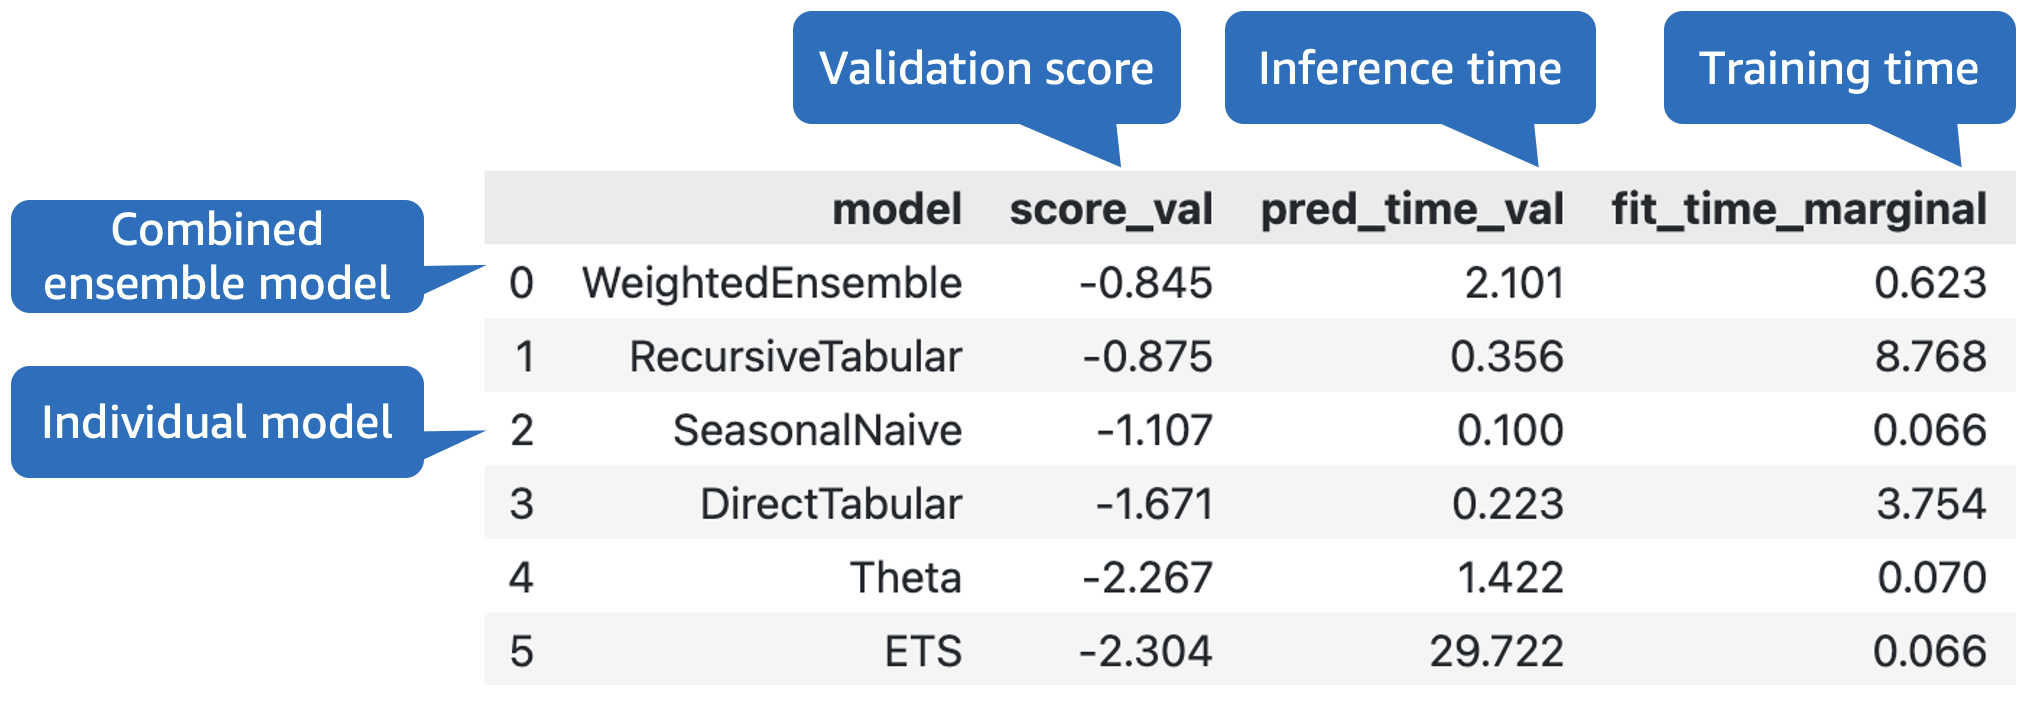
\includegraphics[width=\linewidth]{timeseries/images/leaderboard.png}

\vfill\null
\columnbreak
% ========================================================================

\section*{Predicting}
Forecast \texttt{prediction\_length} steps into the future starting from the end of each time series in \texttt{train\_data}.
\begin{minted}[fontsize=\footnotesize, bgcolor=codeback, frame=leftline, framesep=10pt]{python}
predictions = predictor.predict(
    train_data,
    # only necessary if known_covariates_names
    # were provided when creating predictor
    known_covariates=known_covariates,
)
known_covariates.head()
\end{minted}
\vspace{-5mm}
\begin{center}
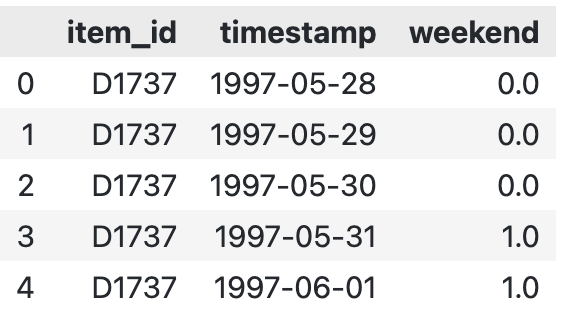
\includegraphics[width=0.35\linewidth]{timeseries/images/future_known_covariates.png}
\end{center}

\medskip

AutoGluon generated probabilistic forecasts that include
\begin{itemize}
    \item mean forecast --- expected value of the time series
    \item quantile forecast --- range of possible outcomes
\end{itemize}

\begin{center}
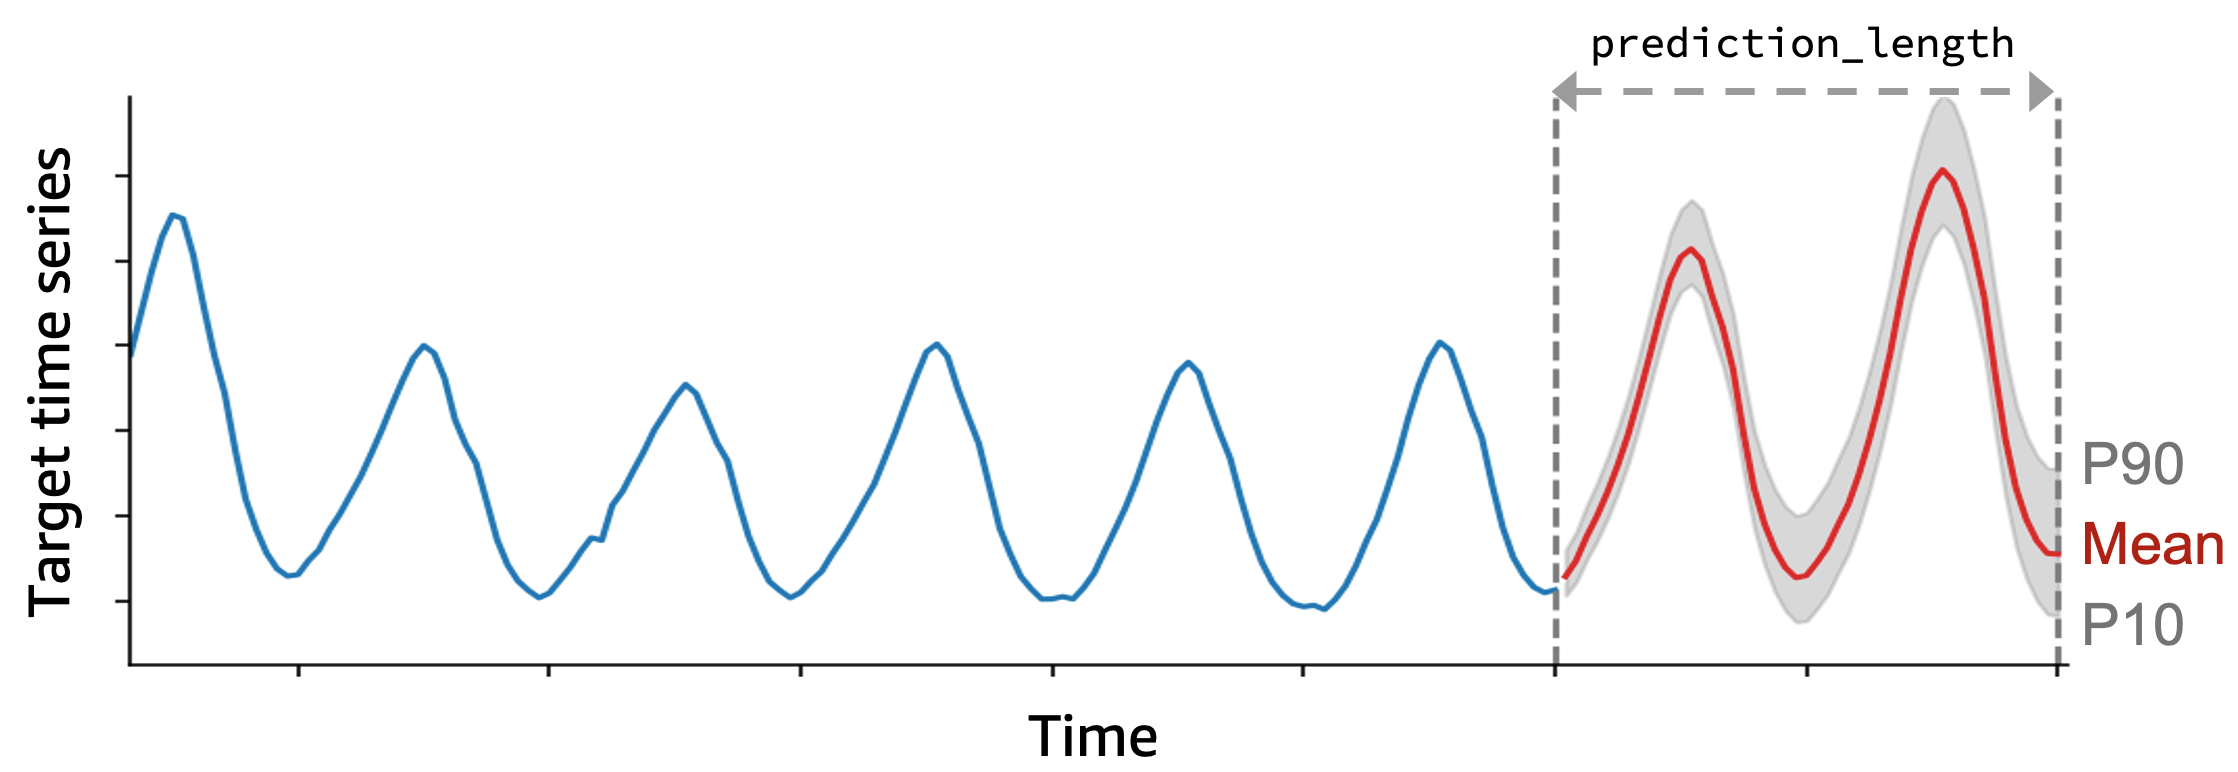
\includegraphics[width=0.95\linewidth]{timeseries/images/probabilistic_forecast.png}
\end{center}

\begin{minted}[fontsize=\footnotesize, bgcolor=codeback, frame=leftline, framesep=10pt]{python}
predictions.head()
\end{minted}

\begin{center}
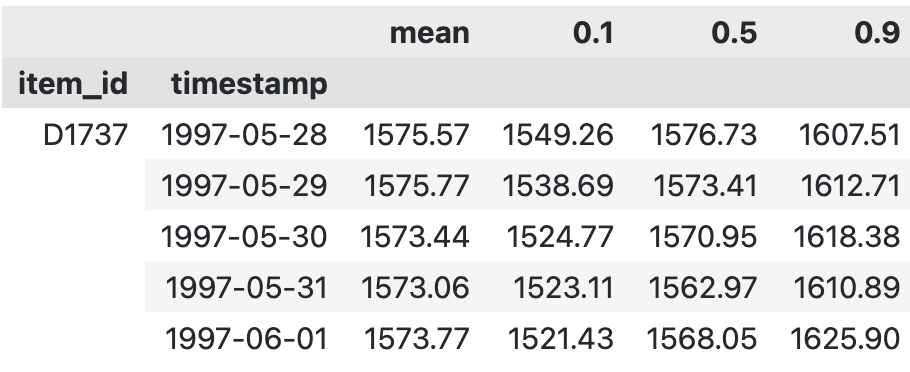
\includegraphics[width=0.6\linewidth]{timeseries/images/predictions.png}
\end{center}

\medskip

AutoGluon predicts with the final ensemble model. You can also predict using an individual model. 

\begin{minted}[fontsize=\footnotesize, bgcolor=codeback, frame=leftline, framesep=10pt]{python}
models = predictor.model_names()
predictor.predict(test_data, model=models[1])
\end{minted}




\begin{itemize}
  \item \href{https://auto.gluon.ai/stable/tutorials/timeseries/index.html}{Detailed  time series tutorials}.
  \item For other types of data, check
  \href{https://auto.gluon.ai/stable/tutorials/tabular/index.html}{TabularPredictor} for tabular data and 
  \href{https://auto.gluon.ai/stable/tutorials/multimodal/index.html}{MultiModalPredictor} for multi-modal data such as images and text. 
  \item Check the \href{https://auto.gluon.ai/stable/cheatsheet.html}{latest version of this cheat sheet}.
  \item Any questions? \href{https://github.com/autogluon/autogluon/discussions}{Ask here}
  \item Like what you see? Consider \href{https://github.com/autogluon/autogluon/stargazers}{starring AutoGluon on GitHub} and \href{https://twitter.com/autogluon}{following us on Twitter} to get notified of the latest updates!
\end{itemize}

% ========================================================================

\raggedcolumns


% \begin{minted}[fontsize=\footnotesize, bgcolor=codeback, frame=leftline, framesep=10pt]{python}
% \end{minted}

% % ========================================================================
\section*{Installation}
\href{https://auto.gluon.ai/stable/index.html}{AutoGluon} (\href{https://github.com/autogluon/autogluon/}{GitHub}) supports Python 3.9 to 3.12 and is available for Linux, MacOS, and Windows. The fastest way to install AutoGluon is through the \href{https://docs.astral.sh/uv/}{uv package manager}.

\begin{minted}[fontsize=\footnotesize, bgcolor=codeback, frame=leftline, framesep=10pt]{bash}
# Install UV package installer (faster than pip)
pip install -U uv
# Install AutoGluon
python -m uv pip install autogluon
\end{minted}

% ========================================================================

\section*{Preparing Data}

AutoGluon can generate forecasts for datasets consisting of \textbf{multiple univariate} time series. Here we use the \href{https://www.sciencedirect.com/science/article/pii/S0169207019301128}{M4 Competition} Daily dataset to demonstrate how to do forecasting with AutoGluon.

\begin{minted}[fontsize=\footnotesize, bgcolor=codeback, frame=leftline, framesep=10pt]{python}
import pandas as pd
raw_data = pd.read_csv("m4_daily.csv")
raw_data.head()
\end{minted}

\begin{center}
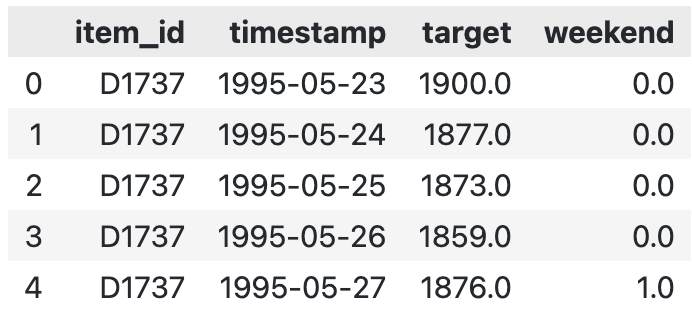
\includegraphics[width=0.6\linewidth]{timeseries/images/raw_data.png}
\end{center}

\medskip

Each row contains unique ID of each time series, timestamp, value of the time series, and (optional) time-varying \textbf{covariates}.

\medskip

A time series datasets may also optionally include time-independent \textbf{static features} (metadata) for each time series.

\begin{minted}[fontsize=\footnotesize, bgcolor=codeback, frame=leftline, framesep=10pt]{python}
static_features = pd.read_csv("m4_metadata.csv")
static_features.head()
\end{minted}

\begin{center}
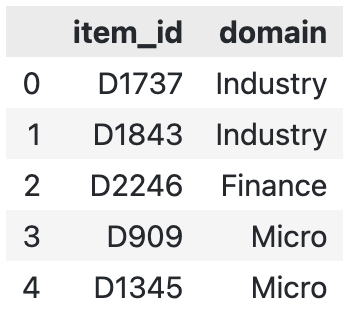
\includegraphics[width=0.30\linewidth]{timeseries/images/static_features.png}
\end{center}

\medskip

We convert raw data into a \textbf{TimeSeriesDataFrame} used by AutoGluon.

\begin{minted}[fontsize=\footnotesize, bgcolor=codeback, frame=leftline, framesep=10pt]{python}
from autogluon.timeseries import TimeSeriesDataFrame
train_data = TimeSeriesDataFrame.from_data_frame(
    raw_data,
    id_column="item_id",
    timestamp_column="timestamp",
    static_features_df=static_features,  # optional
)
\end{minted}


\vfill\null
\columnbreak
% ========================================================================

\section*{Training}

Train models to forecast the values in the column ‘target’ 30 steps into the future for each time series.

\begin{minted}[fontsize=\footnotesize, bgcolor=codeback, frame=leftline, framesep=10pt]{python}
from autogluon.timeseries import TimeSeriesPredictor
predictor = TimeSeriesPredictor(
    target="target",
    prediction_length=30,
).fit(train_data, presets="medium_quality")
\end{minted}

More options to construct a \textbf{TimeSeriesPredictor} instance (\href{https://auto.gluon.ai/stable/api/autogluon.timeseries.TimeSeriesPredictor.html}{docs}):

\begin{minted}[fontsize=\footnotesize, bgcolor=codeback, frame=leftline, framesep=10pt]{python}
# The metric used to tune models
eval_metric="MASE"
# Select quantiles for the probabilistic forecast
quantile_levels = [0.1, 0.5, 0.9]
# If data has irregular timestamps, provide frequency
freq="D"
# Covariates that are known in the future
# (e.g., holidays, promotions, weather forecasts)
known_covariates_names=["weekend"]
\end{minted}
More options for the \textbf{fit} method (\href{https://auto.gluon.ai/stable/api/autogluon.timeseries.TimeSeriesPredictor.fit.html}{docs}):

\begin{minted}[fontsize=\footnotesize, bgcolor=codeback, frame=leftline, framesep=10pt]{python}
# Limit the training time, in seconds
time_limit=600
# More accurate forecasts but longer training time
presets="best_quality"
# Backtest using multiple validation windows
num_val_windows=3
# Manually select what models to use,
# e.g., only use ETS and Chronos-Bolt (Base)
hyperparameters={
    "ETS": {"seasonal_period": 14},
    "Chronos": {"model_path": "bolt_base"},
}
# Ignore some models
excluded_model_types=["AutoARIMA", "PatchTST"]
\end{minted}



\section*{Monitoring}
Understand the contribution of each model.

\begin{minted}[fontsize=\footnotesize, bgcolor=codeback, frame=leftline, framesep=10pt]{python}
predictor.leaderboard()
\end{minted}

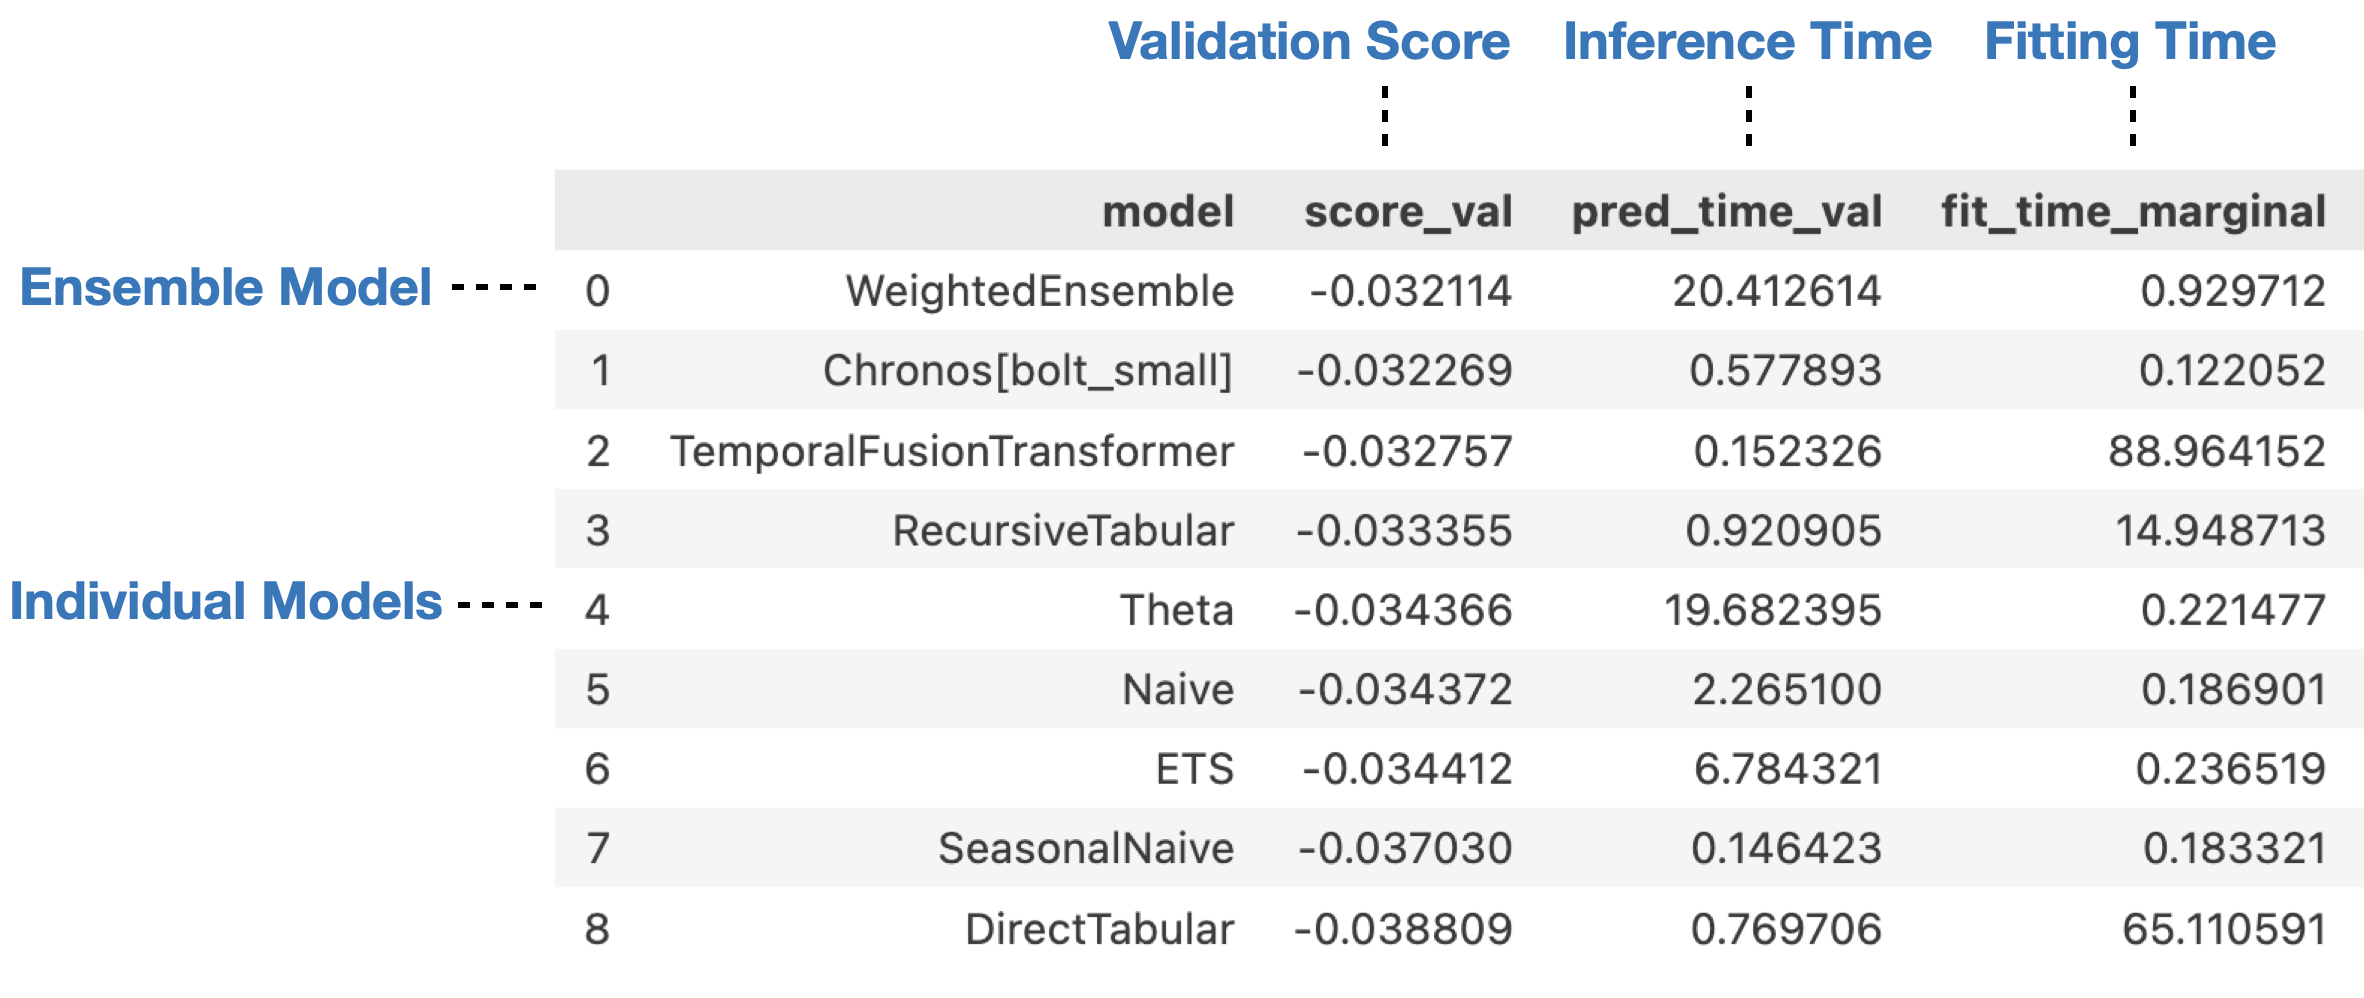
\includegraphics[width=\linewidth]{timeseries/images/leaderboardv1.2-medium_quality.png}

\vfill\null
\columnbreak
% ========================================================================

\section*{Predicting}
Forecast \texttt{prediction\_length} steps into the future starting from the end of each time series in \texttt{train\_data}.
\begin{minted}[fontsize=\footnotesize, bgcolor=codeback, frame=leftline, framesep=10pt]{python}
predictions = predictor.predict(
    train_data,
    # only necessary if known_covariates_names
    # were provided when creating predictor
    known_covariates=known_covariates,
)
known_covariates.head()
\end{minted}
\vspace{-5mm}
\begin{center}
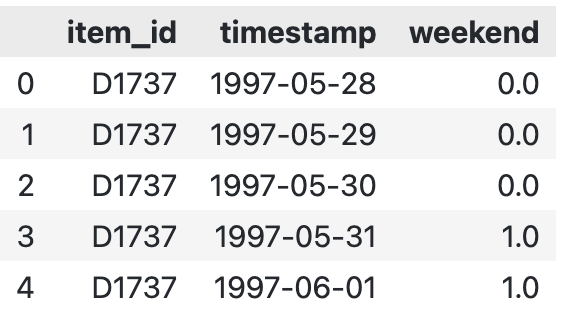
\includegraphics[width=0.35\linewidth]{timeseries/images/future_known_covariates.png}
\end{center}

\medskip

AutoGluon generated probabilistic forecasts that include
\begin{itemize}
    \item mean forecast --- expected value of the time series
    \item quantile forecast --- range of possible outcomes
\end{itemize}

\begin{center}
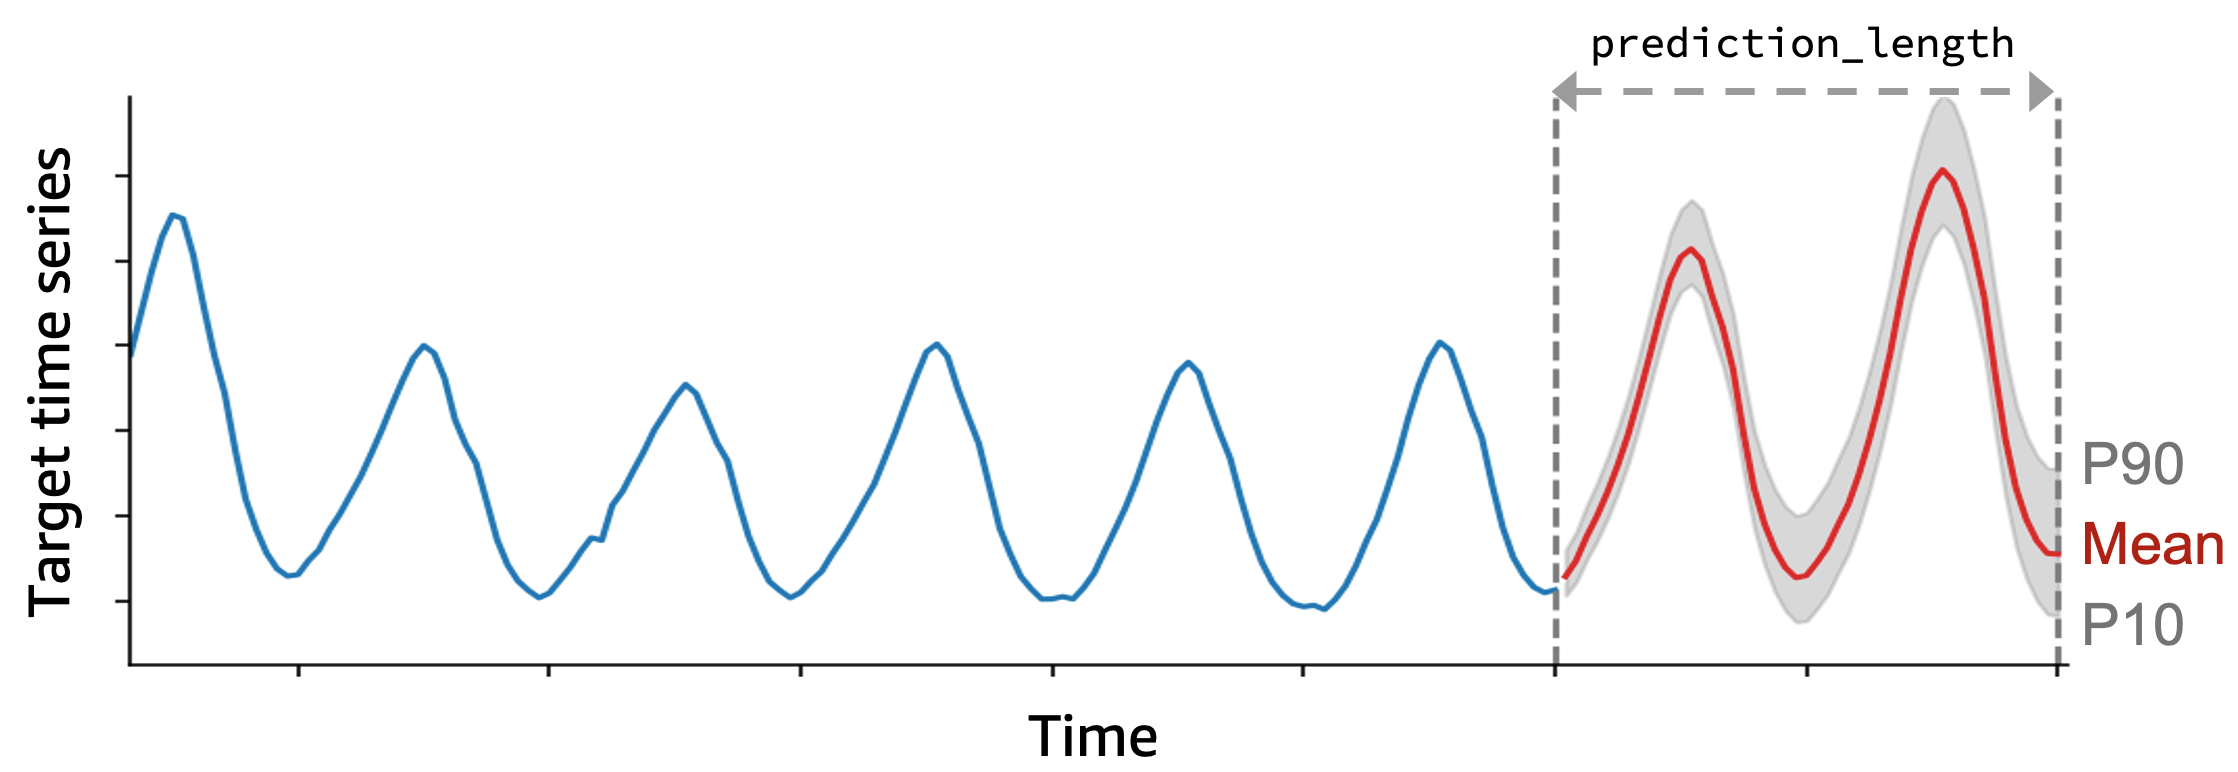
\includegraphics[width=0.95\linewidth]{timeseries/images/probabilistic_forecast.png}
\end{center}

\begin{minted}[fontsize=\footnotesize, bgcolor=codeback, frame=leftline, framesep=10pt]{python}
predictions.head()
\end{minted}

\begin{center}
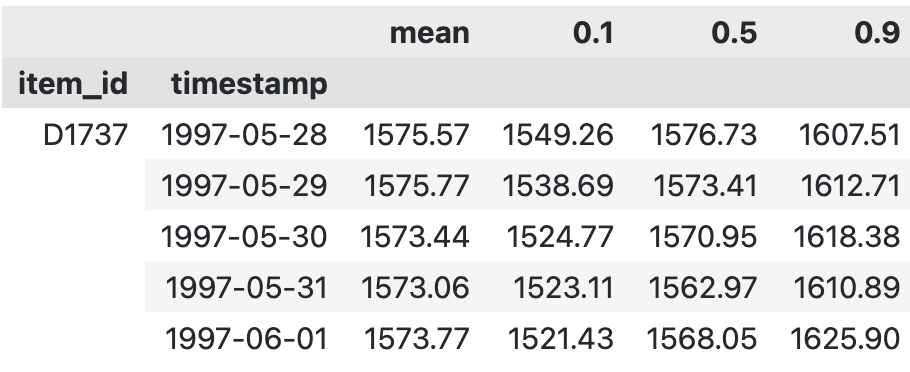
\includegraphics[width=0.6\linewidth]{timeseries/images/predictions.png}
\end{center}

\medskip

AutoGluon predicts with the final ensemble model. You can also predict using an individual model. 

\begin{minted}[fontsize=\footnotesize, bgcolor=codeback, frame=leftline, framesep=10pt]{python}
models = predictor.model_names()
predictor.predict(test_data, model=models[1])
\end{minted}




\begin{itemize}
  \item \href{https://auto.gluon.ai/stable/tutorials/timeseries/index.html}{Detailed  time series tutorials}.
  \item For other types of data, check
  \href{https://auto.gluon.ai/stable/tutorials/tabular/index.html}{TabularPredictor} for tabular data and 
  \href{https://auto.gluon.ai/stable/tutorials/multimodal/index.html}{MultiModalPredictor} for multi-modal data such as images and text. 
  \item Check the \href{https://auto.gluon.ai/stable/cheatsheet.html}{latest version of this cheat sheet}.
  \item Any questions? \href{https://github.com/autogluon/autogluon/discussions}{Ask here}
  \item Like what you see? Consider \href{https://github.com/autogluon/autogluon/stargazers}{starring AutoGluon on GitHub} and \href{https://twitter.com/autogluon}{following us on X (Twitter)} to get notified of the latest updates!
\end{itemize}

% ========================================================================

\raggedcolumns


% \begin{minted}[fontsize=\footnotesize, bgcolor=codeback, frame=leftline, framesep=10pt]{python}
% \end{minted}

% ========================================================================
\section*{Installation}
\href{https://auto.gluon.ai/stable/index.html}{AutoGluon} (\href{https://github.com/autogluon/autogluon/}{GitHub}) supports Python 3.9 to 3.12 and is available for Linux, MacOS, and Windows. The fastest way to install AutoGluon is through the \href{https://docs.astral.sh/uv/}{uv package manager}.

\begin{minted}[fontsize=\footnotesize, bgcolor=codeback, frame=leftline, framesep=10pt]{bash}
# Install uv package installer (faster than pip)
python -m pip install -U uv
# Install AutoGluon
python -m uv pip install autogluon
\end{minted}

% ========================================================================

\section*{Preparing Data}

AutoGluon can generate forecasts for datasets consisting of \textbf{multiple univariate} time series. Here we use the \href{https://www.sciencedirect.com/science/article/pii/S0169207019301128}{M4 Competition} Daily dataset to demonstrate how to do forecasting with AutoGluon.

\begin{minted}[fontsize=\footnotesize, bgcolor=codeback, frame=leftline, framesep=10pt]{python}
import pandas as pd
raw_data = pd.read_csv("m4_daily.csv")
raw_data.head()
\end{minted}

\begin{center}
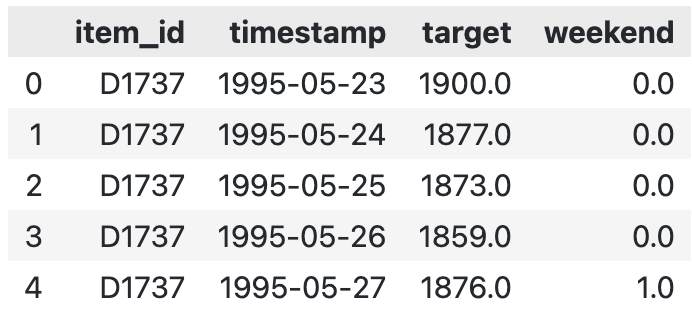
\includegraphics[width=0.6\linewidth]{timeseries/images/raw_data.png}
\end{center}

\medskip

Each row contains unique ID of each time series, timestamp, value of the time series, and (optional) time-varying \textbf{covariates}.

\medskip

A time series datasets may also optionally include time-independent \textbf{static features} (metadata) for each time series.

\begin{minted}[fontsize=\footnotesize, bgcolor=codeback, frame=leftline, framesep=10pt]{python}
static_features = pd.read_csv("m4_metadata.csv")
static_features.head()
\end{minted}

\begin{center}
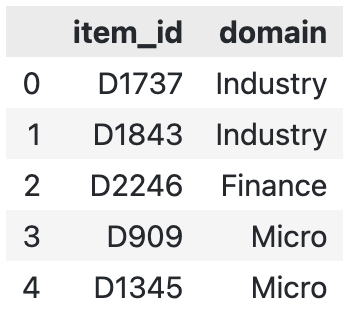
\includegraphics[width=0.30\linewidth]{timeseries/images/static_features.png}
\end{center}

\medskip

We convert raw data into a \textbf{TimeSeriesDataFrame} used by AutoGluon.

\begin{minted}[fontsize=\footnotesize, bgcolor=codeback, frame=leftline, framesep=10pt]{python}
from autogluon.timeseries import TimeSeriesDataFrame
train_data = TimeSeriesDataFrame.from_data_frame(
    raw_data,
    id_column="item_id",
    timestamp_column="timestamp",
    static_features_df=static_features,  # optional
)
\end{minted}


\vfill\null
\columnbreak
% ========================================================================

\section*{Training}

Train models to forecast the values in the column ‘target’ 30 steps into the future for each time series.

\begin{minted}[fontsize=\footnotesize, bgcolor=codeback, frame=leftline, framesep=10pt]{python}
from autogluon.timeseries import TimeSeriesPredictor
predictor = TimeSeriesPredictor(
    target="target",
    prediction_length=30,
).fit(train_data, presets="medium_quality")
\end{minted}

More options to construct a \textbf{TimeSeriesPredictor} instance (\href{https://auto.gluon.ai/stable/api/autogluon.timeseries.TimeSeriesPredictor.html}{docs}):

\begin{minted}[fontsize=\footnotesize, bgcolor=codeback, frame=leftline, framesep=10pt]{python}
# The metric used to tune models
eval_metric="MASE"
# Select quantiles for the probabilistic forecast
quantile_levels = [0.1, 0.5, 0.9]
# If data has irregular timestamps, provide frequency
freq="D"
# Covariates that are known in the future
# (e.g., holidays, promotions, weather forecasts)
known_covariates_names=["weekend"]
\end{minted}
More options for the \textbf{fit} method (\href{https://auto.gluon.ai/stable/api/autogluon.timeseries.TimeSeriesPredictor.fit.html}{docs}):

\begin{minted}[fontsize=\footnotesize, bgcolor=codeback, frame=leftline, framesep=10pt]{python}
# Limit the training time, in seconds
time_limit=600
# More accurate forecasts but longer training time
presets="best_quality"
# Backtest using multiple validation windows
num_val_windows=3
# Manually select what models to use,
# e.g., only use ETS and Chronos-Bolt (Base)
hyperparameters={
    "ETS": {"seasonal_period": 14},
    "Chronos": {"model_path": "bolt_base"},
}
# Ignore some models
excluded_model_types=["AutoARIMA", "PatchTST"]
\end{minted}



\section*{Monitoring}
Understand the contribution of each model.

\begin{minted}[fontsize=\footnotesize, bgcolor=codeback, frame=leftline, framesep=10pt]{python}
predictor.leaderboard()
\end{minted}

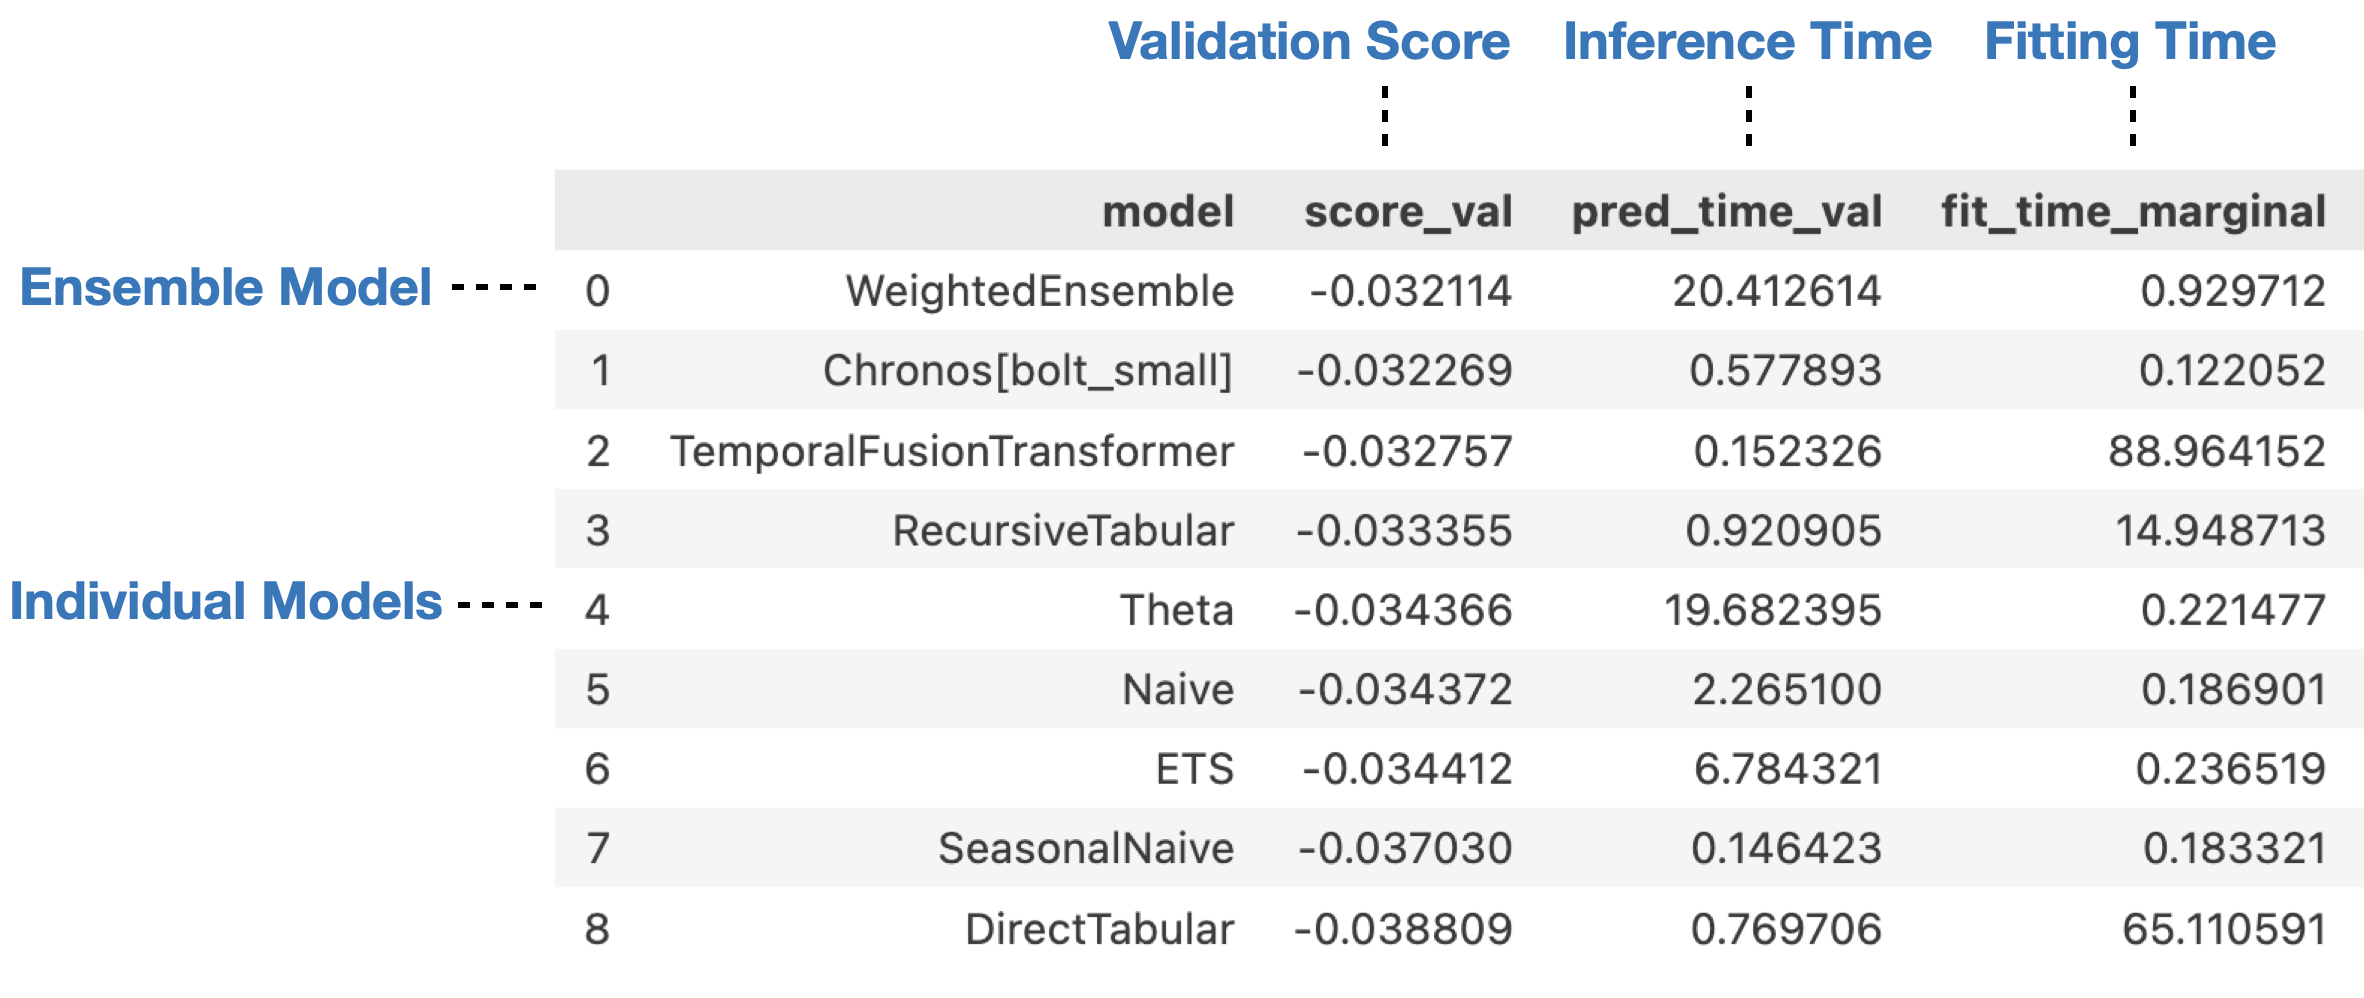
\includegraphics[width=\linewidth]{timeseries/images/leaderboardv1.2-medium_quality.png}

\vfill\null
\columnbreak
% ========================================================================

\section*{Predicting}
Forecast \texttt{prediction\_length} steps into the future starting from the end of each time series in \texttt{train\_data}.
\begin{minted}[fontsize=\footnotesize, bgcolor=codeback, frame=leftline, framesep=10pt]{python}
predictions = predictor.predict(
    train_data,
    # only necessary if known_covariates_names
    # were provided when creating predictor
    known_covariates=known_covariates,
)
known_covariates.head()
\end{minted}
\vspace{-5mm}
\begin{center}
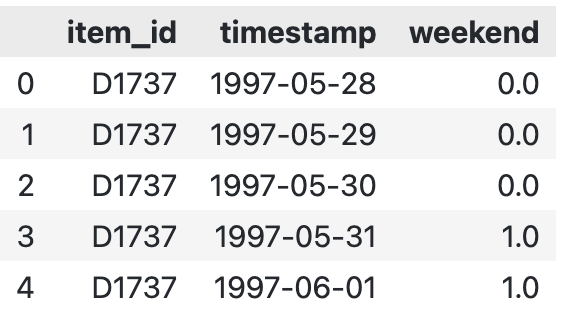
\includegraphics[width=0.35\linewidth]{timeseries/images/future_known_covariates.png}
\end{center}

\medskip

AutoGluon generated probabilistic forecasts that include
\begin{itemize}
    \item mean forecast --- expected value of the time series
    \item quantile forecast --- range of possible outcomes
\end{itemize}

\begin{center}
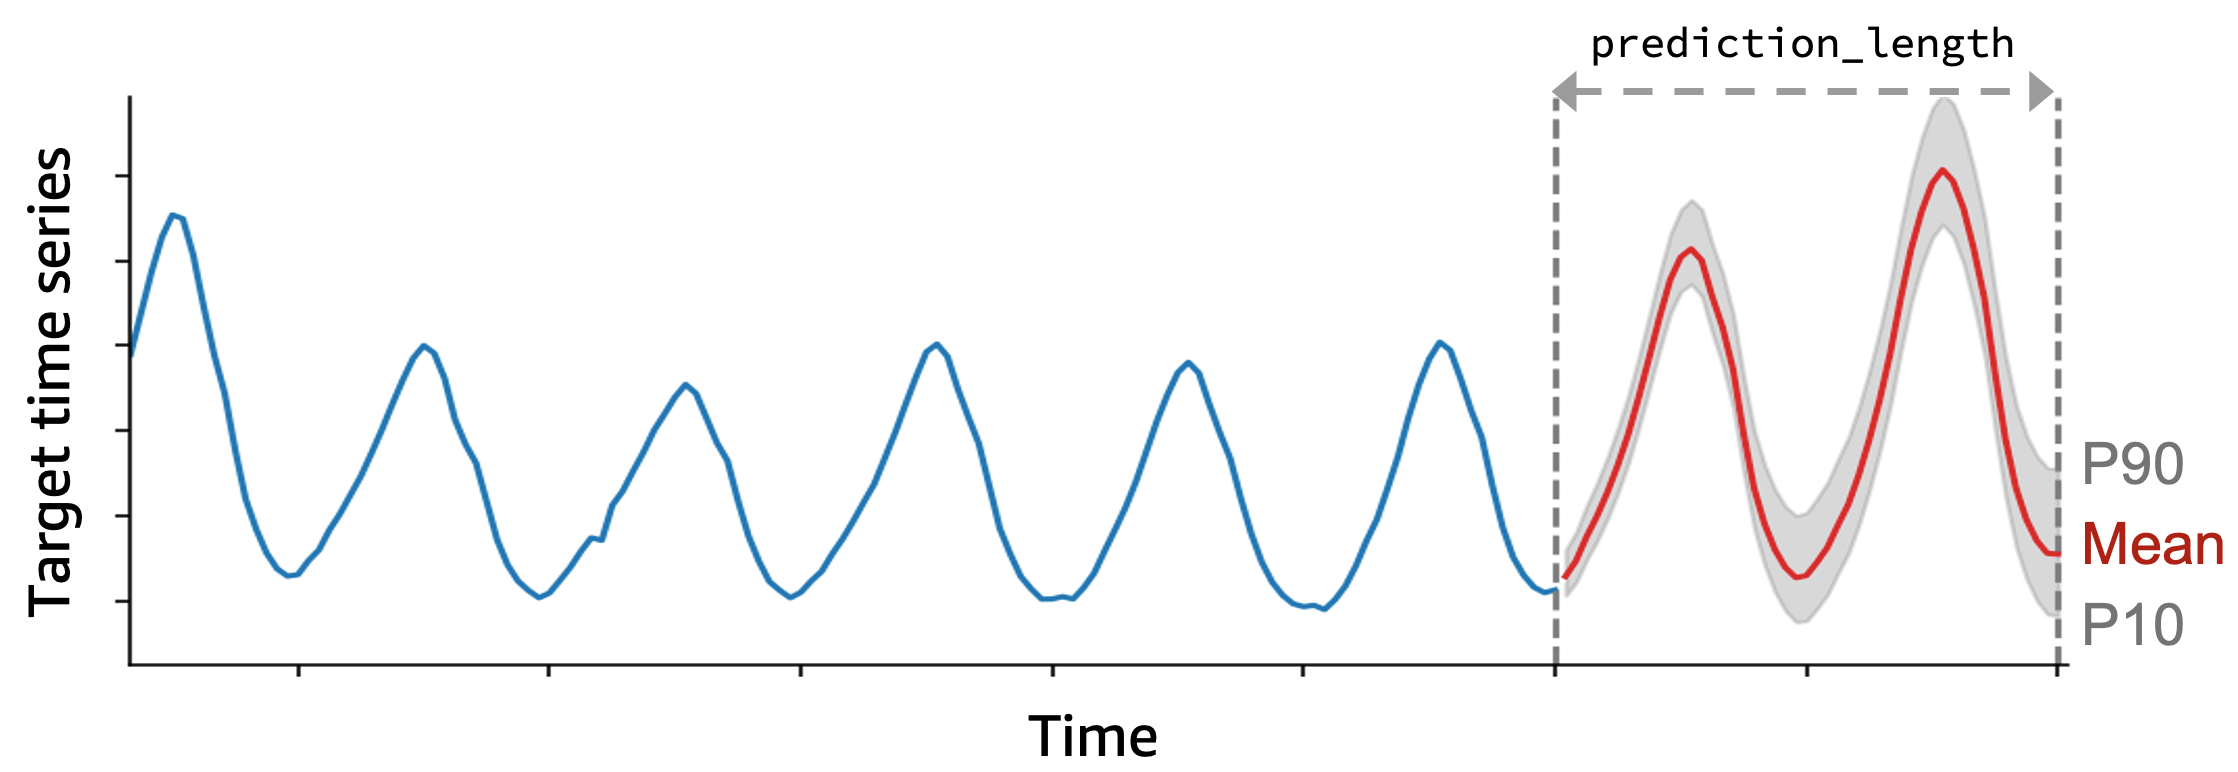
\includegraphics[width=0.95\linewidth]{timeseries/images/probabilistic_forecast.png}
\end{center}

\begin{minted}[fontsize=\footnotesize, bgcolor=codeback, frame=leftline, framesep=10pt]{python}
predictions.head()
\end{minted}

\begin{center}
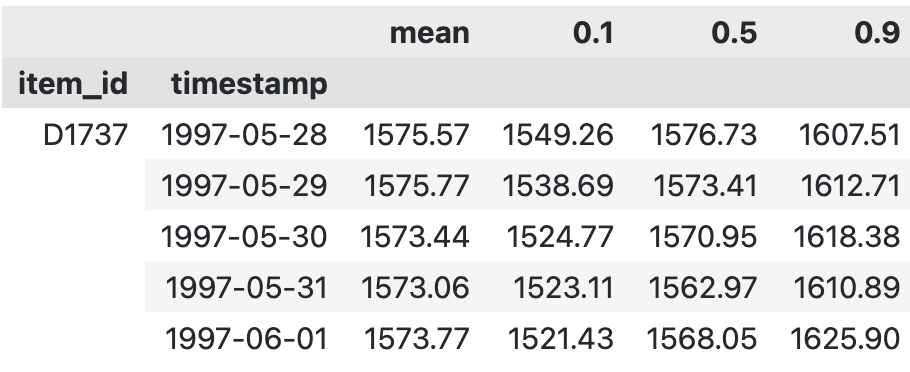
\includegraphics[width=0.6\linewidth]{timeseries/images/predictions.png}
\end{center}

\medskip

AutoGluon predicts with the final ensemble model. You can also predict using an individual model. 

\begin{minted}[fontsize=\footnotesize, bgcolor=codeback, frame=leftline, framesep=10pt]{python}
models = predictor.model_names()
predictor.predict(test_data, model=models[1])
\end{minted}




\begin{itemize}
  \item \href{https://auto.gluon.ai/stable/tutorials/timeseries/index.html}{Detailed  time series tutorials}.
  \item For other types of data, check
  \href{https://auto.gluon.ai/stable/tutorials/tabular/index.html}{TabularPredictor} for tabular data and 
  \href{https://auto.gluon.ai/stable/tutorials/multimodal/index.html}{MultiModalPredictor} for multi-modal data such as images and text. 
  \item Check the \href{https://auto.gluon.ai/stable/cheatsheet.html}{latest version of this cheat sheet}.
  \item Any questions? \href{https://github.com/autogluon/autogluon/discussions}{Ask here}
  \item Like what you see? Consider \href{https://github.com/autogluon/autogluon/stargazers}{starring AutoGluon on GitHub} and \href{https://twitter.com/autogluon}{following us on X (Twitter)} to get notified of the latest updates!
\end{itemize}

% ========================================================================

\raggedcolumns


% \begin{minted}[fontsize=\footnotesize, bgcolor=codeback, frame=leftline, framesep=10pt]{python}
% \end{minted}


\end{multicols*}
\end{document}